\documentclass[12pt, a4paper]{ctexart}

% 基本宏包
\usepackage{amsmath, amssymb}
\usepackage{graphicx}
\usepackage{float}
\usepackage{booktabs}
\usepackage{geometry}
\usepackage{caption}
\usepackage{fancyhdr}
\usepackage[hidelinks]{hyperref}
\usepackage{cite}
\usepackage{multirow}
\usepackage{tabularx}
\usepackage{listings}
\usepackage{xcolor}
\usepackage{tocloft}
% \usepackage[round]{natbib}

% 定义 VS Code 深色主题配色
\definecolor{light-bg}{rgb}{1,1,1} % 背景色(白色)
\definecolor{light-fg}{rgb}{0,0,0} % 默认前景色(黑色)
\definecolor{light-keyword}{rgb}{0.1,0.1,0.8} % 关键字颜色(深蓝色)
\definecolor{light-string}{rgb}{0.2,0.6,0.2}  % 字符串颜色(绿色)
\definecolor{light-comment}{rgb}{0.5,0.5,0.5} % 注释颜色(灰色)
\definecolor{light-number}{rgb}{0.8,0.2,0.2}  % 数字颜色(红色)
\definecolor{light-function}{rgb}{0.1,0.5,0.8} % 函数名颜色(蓝色)
\definecolor{light-type}{rgb}{0.6,0.4,0.2}    % 类型颜色(棕色)
\definecolor{light-constant}{rgb}{0.1,0.1,0.1} % 常量颜色(深灰色)

% 全局代码样式设置
\lstset{
    backgroundcolor=\color{light-bg},   % 背景颜色(白色)
    basicstyle=\ttfamily\small\color{light-fg}, % 基本字体样式(黑色)
    keywordstyle=\color{light-keyword}\bfseries, % 关键字样式(深蓝色)
    stringstyle=\color{light-string},  % 字符串样式(绿色)
    commentstyle=\color{light-comment}\itshape, % 注释样式(灰色)
    identifierstyle=\color{light-constant}, % 标识符样式(深灰色)
    numbersep=5pt,                    % 行号与代码的间距
    frame=single,                     % 添加边框
    framesep=5pt,                     % 边框与代码的间距
    rulecolor=\color{light-fg},       % 边框颜色(黑色)
    breaklines=true,                  % 自动换行
    breakatwhitespace=false,          % 仅在空格处换行
    showstringspaces=false,           % 不显示字符串中的空格
    tabsize=4,                        % Tab 宽度
    captionpos=b,                     % 标题位置
    moreemph=[2]{def, class, import, from, as, if, else, elif, for, while, return, True, False, None, python3.9,pip,chatchat,ollama,git}, % 自定义关键字
    emphstyle=[2]{\color{light-keyword}\bfseries}, % 自定义关键字样式
}


% 页面设置
\geometry{a4paper, left=3cm, right=2.5cm, top=2.5cm, bottom=2.5cm}
\setlength{\parindent}{2em}
\setlength{\headheight}{14.49998pt} % 设置标题高度
\addtolength{\topmargin}{-2.49998pt} % 可选:调整顶部边距
\linespread{1.5}

\setlength{\cftbeforesecskip}{0pt} % 调整章节之间的间距
\setlength{\cftbeforesubsecskip}{0pt} % 调整子章节之间的间距

% 页眉页脚
\pagestyle{fancy}
\fancyhead[L]{北京大学}
\fancyhead[C]{}
\fancyhead[R]{PolicyBERT:基于全词掩码的中文政策文本预训练语言模型}
\fancyfoot[C]{\thepage}

% 打印中英文标题
\title{
    
\includegraphics[width=0.8\textwidth]{./images/logo.png} \\[1em] % 插入 logo
    {\fontsize{40pt}{24pt}\selectfont \textbf{本科生毕业论文}} \\[2em] % 调整大标题字号
    \textbf{PolicyBERT:基于全词掩码的中文政策文本预训练语言模型} \\[1em]
    PolicyBERT: A Chinese Policy Text Pre-trained Language Model Based on Whole Word Masking  \\[3em] % 英文标题去掉加粗
}


\author{姓名:浦皓天 \\
学号:2100016620 \\
院系:信息管理系 \\
专业:大数据管理与应用 \\
导师姓名:孟凡}

% 日期置于页面底部
\date{}

\begin{document}

\maketitle
\vfill
\begin{center}
    \textbf{二〇二五 年 五 月} \\[1em] % 日期格式
\end{center}

\newpage
\begin{center}
    \textbf{\LARGE 北京大学本科毕业论文导师评阅表}
\end{center}

\vspace{1em}

\renewcommand{\arraystretch}{1.5} % 设置行高
\begin{tabularx}{0.87\textwidth}{|X|X|X|X|}
    \hline
    学生姓名 &   & 学号 &  \\
    \hline
    院系 &   & 专业 &  \\
    \hline
    指导教师 &    & 职称 & \\
    \hline
    毕业论文题目 & \multicolumn{3}{l|}{} \\
    \hline
    导师是否同意参加毕业论文答辩 & &建议成绩(可选填) & \\
    \hline
    \vspace{3cm} 导师评语 \newline \rule{0pt}{10cm} & \multicolumn{3}{|p{0.6\textwidth}|}{(包括但不限于对论文选题意义、行文逻辑、专业素养、学术规范以及是否符合培养方案目标等方面评价)\newline \rule{0pt}{12cm} \vfill  导师签名:\hspace{2.5cm} \underline{\hspace{1.5cm}} 年 \underline{\hspace{0.5cm}} 月 \underline{\hspace{0.5cm}} 日} \\ 
    \hline
\end{tabularx}

\newpage
\section*{摘要}
本文提出了一种基于融合式中文编码模型的文本编码器——PolicyBERT,旨在提升中文政策文本的语义理解与生成能力。通过引入HanLP分词、门控机制和多头注意力机制,PolicyBERT能够有效融合字符级和词级信息,增强对中文政策文本的建模能力。本文在多个任务与公开数据集上进行了对比实验,实验结果表明,PolicyBERT在多个任务上均表现出色,尤其是在中文分词(CWS)和词性标注(POS)任务中,分别达到了0.9816和0.9716的F1值,显著优于其他模型。此外,在句子对匹配(SPM)任务中,PolicyBERT的多头注意力机制融合方法取得了0.9016的最高F1值,显示出其在捕捉上下文语义关系方面的优势。本文构建了两个适用于中文政策文本的下一句预测(NSP)任务数据集(PolicySM-1和PolicySM-2),并在这些数据集上进行了模型微调。实验结果表明,使用多头注意力机制的模型在NSP任务中表现最佳,达到了0.9325的准确率。此外,本文基于微调后的模型,使用Ollama与langchain-chatchat架构搭建了一个基于检索增强生成(RAG)机制的智能问答系统“未名问政”,实现了从文本检索到问答生成的全流程部署。该系统具备部署灵活、响应快速、扩展便捷等特点,适用于政务智能问答、政策知识库构建与自动解读等场景。本文的研究为中文政策文本处理提供了新的方法和工具,具有重要的理论意义和实际应用价值。

\vspace{2em} % 添加空行

\textbf{关键词:}中文政策文本,融合式编码模型,PolicyBERT,分词,检索增强生成,未名问政
\vspace{2em} % 添加空行

\newpage
\section*{Abstract}
This paper proposes a text encoder, PolicyBERT, based on a fusion-based Chinese encoding model, aiming to enhance the semantic understanding and generation capabilities of Chinese policy texts. By introducing HanLP word segmentation, gating mechanisms, and multi-head attention mechanisms, PolicyBERT effectively integrates character-level and word-level information, improving its modeling capabilities for Chinese policy texts. Comparative experiments were conducted on multiple tasks and public datasets, and the results demonstrate that PolicyBERT performs exceptionally well across various tasks. Specifically, it achieved F1 scores of 0.9816 and 0.9716 in Chinese Word Segmentation (CWS) and Part-of-Speech Tagging (POS) tasks, respectively, significantly outperforming other models. Additionally, in the Sentence Pair Matching (SPM) task, the multi-head attention mechanism fusion method of PolicyBERT achieved the highest F1 score of 0.9016, showcasing its advantages in capturing contextual semantic relationships. This paper also constructed two datasets for Next Sentence Prediction (NSP) tasks tailored to Chinese policy texts (PolicySM-1 and PolicySM-2) and fine-tuned the model on these datasets. Experimental results show that models using the multi-head attention mechanism performed best in the NSP task, achieving an accuracy of 0.9325. Furthermore, based on the fine-tuned model, this paper developed an intelligent question-answering system, "WeiMing Policy Q\&A," using the Ollama and langchain-chatchat architecture, which is based on a Retrieval-Augmented Generation (RAG) mechanism. This system achieves end-to-end deployment from text retrieval to answer generation and features flexible deployment, fast response, and easy scalability, making it suitable for scenarios such as intelligent government Q\&A, policy knowledge base construction, and automatic interpretation. This research provides new methods and tools for processing Chinese policy texts, with significant theoretical and practical value.



\vspace{2em} % 添加空行

\textbf{Keywords:} Chinese policy texts, fusion-based encoding model, PolicyBERT, word segmentation, Retrieval-Augmented Generation, WeiMing Policy Q\&A

\newpage
\renewcommand{\cfttoctitlefont}{\hfill\Huge\bfseries} % 设置标题字体和大小
\renewcommand{\cftaftertoctitle}{\hfill} % 设置标题居中
\tableofcontents % 目录另起一页
\thispagestyle{fancy}
\newpage


\section{引言}
自然语言处理(Natural Language Processing,NLP)是人工智能领域的重要分支,旨在使计算机能够理解、分析和生成自然语言。随着互联网的快速发展,海量文本数据的产生为 NLP 研究提供了丰富的资源,同时也带来了新的挑战。尤其是在中文文本处理方面,由于汉字的独特性和复杂性,传统的基于词典的方法难以满足实际需求。因此,如何有效地表示和理解中文文本成为了一个亟待解决的问题。

在自然语言处理的早期,文本表示主要依赖于基于词典的特征工程方法,如 TF-IDF 通过词频和逆文档频率量化词的重要性\cite{SALTON1988513},主题模型(如 LDA)则挖掘文本的潜在主题分布,将文档映射到低维主题向量空间,提升了语义理解能力\cite{10.5555/944919.944937}。随着深度学习的兴起,分布式词向量技术(如 Word2Ve\cite{mikolov2013efficientestimationwordrepresentations} 和 GloVe\cite{pennington-etal-2014-glove})通过大规模无标注语料训练,将词映射为低维实数向量,捕捉词间相似性,但其“静态”表示难以区分多义词,对上下文变化不敏感。为此,ELMo 引入了基于双向语言模型的上下文相关表示,使同一词在不同上下文中具有不同向量,显著提升了下游任务性能\cite{peters-etal-2018-deep}。

基于 Transformer 架构的预训练语言模型(PLM)带来了革命性变革。BERT 首创了“掩码语言模型”和“下游任务微调”范式,通过海量语料预训练并在具体任务上微调,大幅提升性能,奠定了通用 NLP 研究的基础\cite{devlin-etal-2019-bert}。其后,RoBERTa 通过更大规模语料和更长训练时间刷新了多项任务表现\cite{liu2019robertarobustlyoptimizedbert},ERNIE 则融入知识图谱与实体信息,在预训练中引入外部知识,进一步增强了语义理解能力\cite{sun2019ernieenhancedrepresentationknowledge}。

尽管上述预训练模型在英文 NLP 任务中表现优异,直接迁移到中文时却面临语言结构层面的挑战。中文语言天然缺乏空格作为词语边界标记,模型在对文本进行编码前通常需先进行分词处理。但中文的词边界存在模糊性和上下文依赖性,使得不同分词方式可能产生完全不同的语义理解。例如,“北京大学”可被切分为“北京”,“大学”或整体作为专有名词“北京大学”,两者所表达的语义截然不同。这种分词歧义会导致 token 级别的预训练模型无法准确建模真实语义。

现有中文 BERT 模型通常采用字符级(字粒度)编码策略,即将每个汉字视为独立 token,这虽然规避了分词带来的歧义问题,但也牺牲了对词语整体语义的把握。例如,将“人工智能”拆解为“人”“工”“智”“能”,使模型需要通过更长的上下文依赖才能捕捉到其作为专有名词的统一语义。这种处理方式尤其不利于处理术语密集、长词多、句式复杂的文本类型。

在 NLP 的具体应用中,领域文本(Domain-specific Text)处理逐渐成为研究热点。尤其是法律、金融、医疗、政策等垂直领域,其文本具有术语密集、专业性强、、结构复杂、长距离依赖、命名实体多、更新频繁等特点,对文本编码提出了更高要求:模型不仅要能理解个体 token 的语义,还要具备对领域词语、命名实体的整体感知能力。这使得纯粹依赖字粒度编码的 BERT 类模型难以充分捕捉政策文本中的关键信息。若模型不能准确识别和建模“国家政策”“财政转移支付”“扶贫开发”等多字短语或专有名词,可能导致信息丢失、下游任务性能下降。

ZEN(a BERT‑based Chinese (Z) text encoder Enhanced by N‑gram representations)提出了引入 n‑gram 表示的中文词信息\cite{diao-etal-2020-zen}。该文使用了Shizhe Diao 等人提出的基于计算相邻字符PMI(Pointwise Mutual Information)的分词方法\cite{DXSJSZ2021}。将所有连续的 n‑gram 片段与字符表示并行编码,并在模型的每一个交叉注意力组件的末尾进行相加融合,以补充多字组合信息。

HanLP 是一个开源的自然语言处理工具包,提供了多种中文分词、词性标注、命名实体识别等功能\cite{he-choi-2021-stem}。其分词器基于 CRF(条件随机场)模型,能够有效处理中文文本中的分词问题。HanLP 的分词器在处理中文文本时,能够根据上下文信息自动选择最优的分词方式,从而提高了分词的准确性和鲁棒性。

本文在 ZEN 的基础上,提出了一种基于融合式中文编码模型的文本编码器——PolicyBERT,旨在提升中文政策文本的语义理解与生成能力。该模型通过使用 HanLP 分词引入了更精准、丰富的词级语义信息,并使用门控与注意力机制提高了模型对词级语义信息的利用能力,增强模型对文本的表示能力。

\vspace{2em} % 添加空行

随着自然语言处理技术的快速发展,基于检索增强生成(Retrieval-Augmented Generation, RAG)的系统架构在政策文本处理领域展现出巨大潜力。RAG是一种将大型语言模型与外部知识库相结合的方法,研究表明,RAG在多个评估指标上优于传统的领域特定微调方法,尤其在知识检索任务中表现出更高的准确性和可靠性\cite{lakatos2024investigatingperformanceretrievalaugmentedgeneration}。政策文本通常具有术语密集、结构复杂、领域专有性强等特点,这对模型的理解和生成能力提出了更高要求。传统的预训练语言模型虽然在通用任务上表现优异,但在特定领域的任务中往往难以充分捕捉领域知识。因此,在子领域上微调过的预训练模型成为解决这一问题的关键,能够更好地适应特定领域的语义需求,提升 RAG 系统的性能。

Ollama 是一个高效的模型部署工具,支持本地化部署大规模语言模型,能够显著降低对外部依赖的需求。本文中,我们使用 Ollama 实现本地部署 $Qwen2.5:7b$,这是一款由阿里巴巴达摩院推出的强大中文语言模型,具备卓越的生成能力和对中文语义的深度理解\cite{qwen2.5}。此外,BGE (BAAI General Embedding) 系列模型在 RAG 任务中表现出色,尤其是 $ bge-base-zh-v1.5 $,其在中文文本嵌入生成方面具有较高的语义一致性和检索精度,为构建高效的检索模块提供了坚实基础\cite{bgeembedding}。

在架构设计上,langchain-chatchat 是一种灵活且高效的框架,专为复杂的 RAG 系统设计,能够无缝集成检索和生成模块,支持多阶段任务处理\cite{langchainchatchat}。langchain-chatchat 的优势在于其模块化设计和对大规模模型的兼容性,使得系统能够在保持高性能的同时,具备良好的扩展性和易用性。

本文将结合 Ollama 部署的 $Qwen2.5:7b$ 和微调后的 $ bge-base-zh-v1.5 $,构建一个高效的 RAG 系统————“未名问政”。该系统将利用本地部署的 $Qwen2.5:7b$ 进行文本生成,并通过使用ZEN架构微调后的 $ bge-base-zh-v1.5 $ 实现高效的政策文本检索与生成任务。通过这一系统,本文验证了在特定领域微调模型和优化架构设计对提升 RAG 系统性能的有效性。

本文的主要贡献包括以下几个方面:提出 PolicyBERT 架构,引入 HanLP 分词、门控与注意力机制,以增强对中文政策文本的建模能力;将 $ bge-base-zh-v1.5 $ 的主体 BERT 部分参数与预训练参数拼接,使用 PolicyBERT 架构进行微调,以适应政策文本的特定需求;使用 Ollama 部署 $Qwen2.5:7b$,并结合 langchain-chatchat 架构构建 RAG 系统,利用微调后的 $ bge-base-zh-v1.5 $,实现高效的政策文本检索与生成任务。通过这一系统,本文验证了多层融合词级信息对文本理解效果的提升,以及在特定领域微调模型和优化架构设计对 RAG 系统性能的提升。本文PolicyBERT的训练和未名问政RAG系统的代码公开在\href{https://github.com/PuHT4213/PolicyBert}{\underline{PuHT4213/PolicyBert}}和\\\href{https://github.com/PuHT4213/WeiMingPolicyRAG}{\underline{PuHT4213/WeiMingPolicyRAG}}上。




\section{相关研究}
ZEN(Pre-training Chinese Text Encoder Enhanced by N-gram Representations)提出了一种专为中文设计的预训练语言模型,旨在解决中文文本处理中的分词不确定性问题\cite{diao-etal-2020-zen}。相较于将每个汉字作为独立token的传统BERT模型,ZEN引入n-gram表示,通过显式建模多粒度的词片段信息,增强了对词级语义的建模能力。在架构上,ZEN在字符级BERT的基础上添加了n-gram编码器,通过融合字符与n-gram表示,有效提升了模型对中文语义结构的理解。实验证明,ZEN在中文分词、命名实体识别、文本分类等多个任务上优于传统方法,表明其多粒度建模策略在中文NLP中具有重要价值。

PTWA(Pre-Training with Word Attention)提出了一个针对中文命名实体识别(NER)任务的预训练方法,旨在更有效地融合词级信息以提升模型性能\cite{Ma2021PTWAPW}。该方法通过引入词注意力机制,增强了字符表示与词级语义之间的交互,从而更准确地识别实体边界和类别。在实验中,PTWA在多个中文NER基准数据集上表现出色,显著优于传统的字符级预训练模型,验证了其在中文NER任务中的有效性和先进性。

Wenbiao Li等人(2022)在其研究《Exploiting Word Semantics to Enrich Character Representations of Chinese Pre-trained Models》中,针对中文预训练语言模型普遍采用字符级建模而忽略词级语义的问题,提出了一种名为“HRMF”(Hidden Representation Mix and Fusion)的新方法\cite{Li2022ExploitingWS}。该方法通过将词嵌入按相似度权重投射到其内部字符嵌入中,增强了字符表示的语义信息。随后,利用字符间的混合机制强化词边界信息,并引入词-字符对齐注意力机制,突出重要字符,抑制不重要字符的影响。此外,为减轻分词错误传播的问题,作者设计了融合多种分词器结果的集成策略。实验结果显示,该方法在情感分类、句子对匹配、自然语言推理和机器阅读理解等任务中,显著优于基础的中文预训练模型如BERT、BERT-wwm和ERNIE,验证了其在丰富字符表示和提升模型性能方面的有效性。

Qiang He等人(2023)在其论文《Prompt-Based Word-Level Information Injection BERT for Chinese Named Entity Recognition》中,提出了一种名为PWII-BERT的模型,旨在提升中文命名实体识别(NER)的性能\cite{He2023PromptBasedWI}。该模型通过引入提示(prompt)机制,将词级信息注入预训练语言模型中,从而更有效地捕捉字符与词之间的关联。具体而言,PWII-BERT设计了一个词级信息注入适配器(WIIA),利用双仿射机制融合字符和词的特征,并在Transformer层中引入类别提示,指导模型关注特定类别的实体信息。实验结果显示,PWII-BERT在四个中文NER基准数据集上均优于现有的主流模型,验证了融合类别信息和词汇特征对于提升中文NER性能的有效性。 



\section{PolicyBERT}
\subsection{研究方法}

\subsubsection{模型输入}
本文提出的 PolicyBERT 的模型架构如图\ref{fig:policybert}所示。其中模型的输入部分由图中左侧所示。

令输入的所有政策文件定义为 
\begin{equation}
    Doc = \{d_1, d_2, \dots, d_{N^{doc}}\} 
\end{equation}

其中 $d_i$ 为第 $i$ 个政策文件,${N^{doc}}$ 为政策文件的总数。我们将每个政策文件 $d_i$ 按照标点、换行符等标识分为$N^{d_i}$个句子。 

\begin{equation}
   d_i = \{s_1, s_2, \dots, s_{N^{d_i}}\} 
\end{equation}

假设每个句子中的词数和字数分别为 $k_w$ 和 $k_c$(暂时不考虑如[UNK]、[CLS]、[SEP]等特殊符号的影响),则每个句子 $s_j$ 可以表示为:
\begin{equation}
    \begin{split}
        s_j &= W_j = C_j \\
        W_j &= \{w_1, w_2, \dots, w_{k_w}\} \\
        C_j &= \{c_1, c_2, \dots, c_{k_c}\}
    \end{split}
\end{equation}

其中 $w_i$ 为第 $i$ 个词,$c_i$ 为第 $i$ 个字。$k_w$ 和 $k_c$ 分别为句子中的词和字符的数量。字符数量 $k_c$ 由句子长度决定。具体对于下游NSP(Next Sentence Prediction)任务,模型输入 $s_j$ 还可以表示为:
\begin{equation}
    \begin{split}
        s_j &= [CLS] + {s_j}^{(1)} + [SEP] + {s_j}^{(2)} + [SEP] \\
    \end{split}
\end{equation} 

为了更好地对应词和字的关系,我们使用一个匹配矩阵(Matching Matrix)${\mathcal{M}}_j  \in N^{k_w \times k_c}$,也即:

${\mathcal{M}}_j$是一个 $k_w \times k_c$ 的0-1矩阵,表示句子中的每一个字是否属于某个词。矩阵的每一行对应一个词 $w_q$,每一列对应一个字 $c_p$。如果字 $c_p$ 属于词 $w_q$,则矩阵中对应位置的值为 1,否则为 0。具体来说,
$ {\mathcal{M}}_j$的每一个元素的取值为:
\begin{equation}
    m_{pq} = \begin{cases}
        1, & \text{if } c_p \in w_q \\
        0, & \text{elif } c_p \notin w_q
    \end{cases}
    \label{eq:matching_matrix}
\end{equation}

实际输入模型时,使用输入句子 $s_j$ 的字符表示$C_j$与词表 $V$ 构建匹配矩阵${\mathcal{M}}_j$和词表示$W_j$。词表 $V$由Hanlp提供的分词接口预先构建,共2662个词。对于$C_j$ ,提取其中的所有存在于 $V$ 的词,记录其索引、起始位置、长度和内容。使用词在词表中的id,可以构建词表示$W_j$:
\begin{equation}
    W_j = \{wid_1, wid_2, \dots, wid_{k_w}\}
\end{equation}
其中 $wid_i$ 为第 $i$ 个词在词表$V$ 中的索引。

同时使用公式\ref{eq:matching_matrix}构建上文提到的匹配矩阵 ${\mathcal{M}}_j$,最后将所有词的顺序打乱,以避免模型学习到词表的顺序信息。每句话的最大词数和最大字符数由超参数${k_w}^{max}$和${k_c^{max}}$决定。对于超过的句子,使用截断(Truncation)处理,保留前 ${k_w}^{max}$ 个词和 ${k_c}^{max}$ 个字符。对于不足的句子,使用零填充(Zero Padding)补齐。如此一来,构成了长度为 ${k_c}^{max}$ 词嵌入$W_j$和长度为 ${k_c}^{max}$ 字嵌入$C_j$。其中 ${k_w}^{max}$ 为预先设定的单个句子中词的最大数量,本文使用${k_w}^{max}=40$;而${k_c}^{max}$ 为预先设定的单个句子中字符的最大数量,本文使用${k_c}^{max}=128$。

由此,我们构建好了模型的全部输入,包括字符表示$C_j$、词表示$W_j$和匹配矩阵${\mathcal{M}}_j$。模型的输入为:
\begin{equation}
        X_j = \{C_j, W_j, {\mathcal{M}}_j\}
\end{equation}

\subsubsection{嵌入、编码与融合}

\begin{figure}
    \centering
    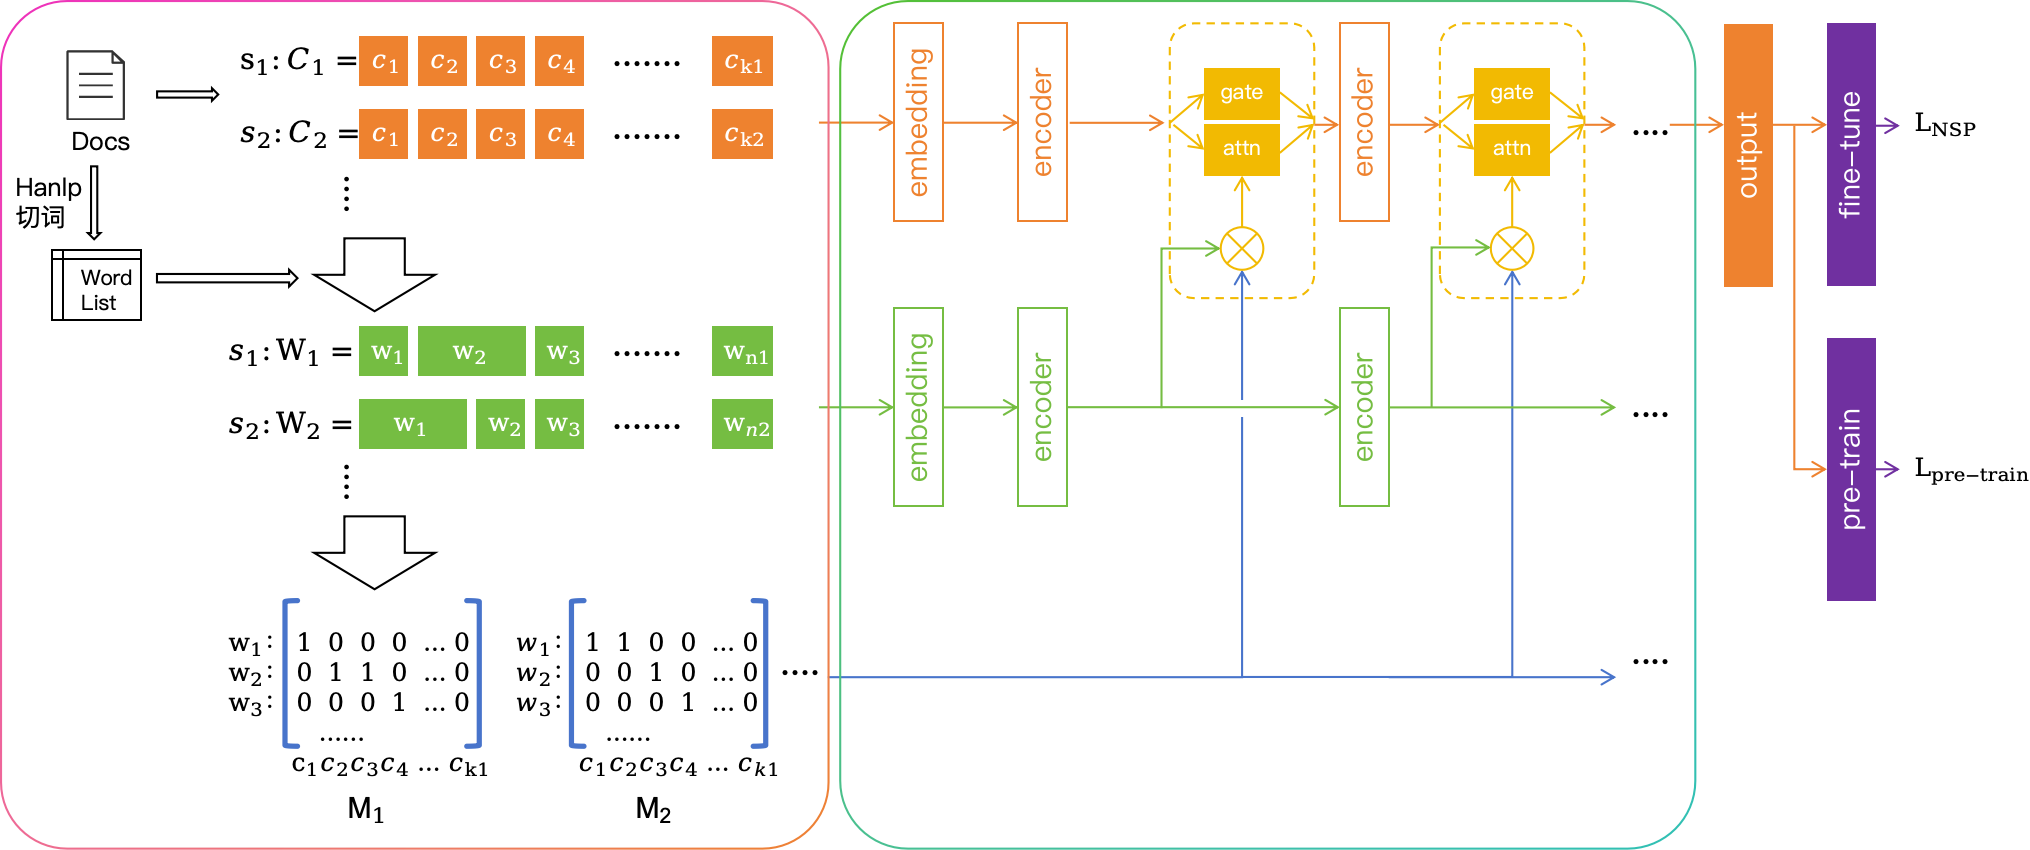
\includegraphics[width=1\textwidth]{./images/model_structure.png}
    \caption{PolicyBERT 模型架构。左侧为模型的输入部分,包括字符表示$C_j$、词表示$W_j$和匹配矩阵${\mathcal{M}}_j$;右侧为模型的主体部分,包括嵌入层、编码层和融合层。其中融合层可以在门控机制和多头注意力机制之间进行切换。}
    \label{fig:policybert}
\end{figure}

模型的主体部分由图\ref{fig:policybert}右侧所示。

模型的输入 $X_j$ 由字符表示 $C_j$、词表示 $W_j$ 和匹配矩阵 ${\mathcal{M}}_j$ 组成。为了将这些输入转换为模型可以处理的向量表示,我们使用了嵌入层(Embedding Layer)、编码层(Encoder)和融合层(Fusion Layer)。

字符表示 $C_j$ 和词表示 $W_j$ 首先通过嵌入层进行转换,得到对应的嵌入向量 $C^{(0)}$ 和 $W^{(0)}$:
\begin{equation}
    \begin{split}
        C^{(0)} &= text\_embedding(C_j) \\
        W^{(0)} &= word\_embedding(W_j) \\
    \end{split}
\end{equation}

用于处理字符输入 $C_j$ 和词输入 $W_j$ 的模型架构相似,均为标准的BERT架构,使用了多层的 Transformer 编码器。
每一层的输入$C^{(l)}$和$W^{(l)}$,经过多头自注意力(Multi-head Self-Attention)处理后,再经过前馈神经网络进行非线性变换。
可以表示为:
\begin{equation}
    \begin{split}
        A^{(l)} &= \text{Attention}(C^{(l)}, \text{mask})\\
        I^{(l)} &= \text{Intermediate}(A^{(l)})\\
        O^{(l)} &= \text{Output}(I^{(l)}, A^{(l)})\\
        C^{(l)}_1 &= O^{(l)} \\
    \end{split}
\end{equation}

对$W^{(l)}$的处理方式类似,只是对于词表示的中间结果$W^{(l)}_1$,会令其与匹配矩阵${\mathcal{M}}_j$进行相乘,得到词表示中间结果$W^{(l)}_2$,而对$C^{(l)}_1$则不进行处理。
\begin{equation}
    \begin{split}
        W^{(l)}_2 &= W^{(l)}_1 \cdot {\mathcal{M}}_j \\
        C^{(l)}_2 &= C^{(l)}_1
    \end{split}
\end{equation}

本文在此基础之上,增加了一个融合层(Fusion Layer),用于将字符和词的表示进行融合。,本文使用了两种融合方式:门控机制(Gated Mechanism)和多头注意力机制(Multi-head Attention Mechanism)。

\vspace{2em} % 添加空行

门控机制:门控机制通过一个包含全连接层(Fully Connected Layer)$Dense$ 、Sigmoid 激活函数和偏置项的门控单元,用字符和词的拼接表示,计算要融合哪些词嵌入的信息。得到新的字符表示 $C^{(l+1)}$:
\begin{equation}
    \begin{split}
        gate^{(l)} &= {\sigma}^{(l)} (Dense(C^{(l)}_2, W^{(l)}_2) ) + b^{(l)} \\
        C^{(l+1)} &= C^{(l)}_2 + gate^{(l)} \cdot W^{(l)}_2 \\
    \end{split}
\end{equation}

其中每个线性层的偏置(bias)被初始化为常数$b^{(0)} = 5.0$,这样通过 sigmoid 激活函数后,初始门控值接近于 1,这意味着初始状态下模型倾向于直接保留字符表示 $C^{(l)}$,与ZEN中直接相加$C^{(l)}_2$和$W^{(l)}_2$的原始方法处在同一出发点。

\vspace{2em} % 添加空行

多头注意力机制:多头注意力机制则是通过计算字符和词的注意力权重,来决定如何融合两者的信息。具体来说,对于每一层的字符表示 $C^{(l)}_2$ 和词表示 $W^{(l)}_2$,多头注意力机制将字符表示作为查询(Query),词表示作为键(Key)和值(Value),输入到多头注意力模块中。通过计算注意力权重,模型能够捕捉字符和词之间的交互关系,从而生成融合后的表示。

具体实现如下:首先,使用字符表示 $C^{(l)}_2$ 作为查询 $Q$,词表示 $W^{(l)}_2$ 作为键 $K$ 和值 $V$,输入到多头注意力模块中:
\begin{equation}
    \text{Attention}(Q, K, V) = \text{softmax}\left(\frac{QK^\top}{\sqrt{d_k}}\right)V
\end{equation}

其中 $d_k$ 是键的维度,用于缩放点积以稳定梯度。

多头注意力机制通过多个独立的注意力头来捕捉不同的特征表示:
\begin{equation}
    \begin{split}
        \text{MultiHead}(Q, K, V) &= \text{Concat}(\text{head}_1, \dots, \text{head}_h)W^O \\
        \text{head}_i &= \text{Attention}(QW_i^Q, KW_i^K, VW_i^V) \\
    \end{split}
\end{equation}

其中 $W_i^Q, W_i^K, W_i^V$ 是每个注意力头的参数矩阵,$W^O$ 是输出的线性变换矩阵。

在融合过程中,模型还引入了残差连接(Residual Connection)和层归一化(Layer Normalization)以增强稳定性:
\begin{equation}
    C^{(l+1)} = \text{LayerNorm}(C^{(l)}_2 + \text{Dropout}(\text{MultiHead}(C^{(l)}_2, W^{(l)}_2, W^{(l)}_2)))
\end{equation}

模型的最后一层输出 $C^{(L)}$,将被用于预训练或下游任务的微调。

\subsubsection{预训练头}
在预训练阶段,模型的最后一层输出 $C^{(L)}$ 被用于两个主要任务:掩码语言模型(Masked Language Model, MLM)和下一句预测(Next Sentence Prediction, NSP)。这两个任务分别用于增强模型的上下文理解能力和句子间关系建模能力。

对于掩码语言模型任务,模型首先对输入序列中的部分 token 进行随机掩码处理(即用特殊标记 [MASK] 替换),然后利用 $C^{(L)}$ 预测这些被掩码的 token。具体来说,$C^{(L)}$ 会被输入到一个语言模型预测头(Language Model Prediction Head)中,该预测头由一个全连接层和 softmax 激活函数组成,用于输出每个被掩码 token 的概率分布。预测的概率分布可以表示为:
\begin{equation}
    P(\hat{y}_i | C^{(L)}) = \text{softmax}(\text{Linear}(C^{(L)}_i))
\end{equation}

其中,$C^{(L)}_i$ 表示第 $i$ 个 token 的隐藏状态,$\hat{y}_i$ 表示模型预测的第 $i$ 个 token 的概率分布。

为了计算 MLM 任务的损失,采用交叉熵损失函数(CrossEntropyLoss),公式如下:
\begin{equation}
    \mathcal{L}_{MLM} = -\frac{1}{N} \sum_{i=1}^{N} y_i \log(\hat{y}_i)
\end{equation}

其中,$N$ 表示被掩码的 token 数量,$y_i$ 表示第 $i$ 个 token 的真实标签,$\hat{y}_i$ 表示模型预测的概率分布。


对于下一句预测任务,模型会将 $C^{(L)}$ 的池化输出(pooled output)输入到一个线性分类器中,用于预测两段句子是否具有连续关系。具体来说,池化操作会提取 $C^{(L)}$ 中 [CLS] 标记对应的隐藏状态,表示为 $C^{(L)}_{\text{[CLS]}}$,然后通过一个线性层映射到二分类的概率空间:
\begin{equation}
    P(\text{NSP} | C^{(L)}) = \text{softmax}(\text{Linear}(C^{(L)}_{\text{[CLS]}}))
\end{equation}

NSP 任务的损失同样采用交叉熵损失函数,公式如下:
\begin{equation}
    \mathcal{L}_{NSP} = -\frac{1}{M} \sum_{j=1}^{M} y_j \log(\hat{y}_j)
\end{equation}

其中,$M$ 表示样本数量,$y_j$ 表示第 $j$ 个样本的真实标签,$\hat{y}_j$ 表示模型预测的概率分布。

最终,预训练阶段的总损失由 MLM 和 NSP 两部分损失相加求和得到:
\begin{equation}
    \mathcal{L}_{\text{pretrain}} = \mathcal{L}_{MLM} + \mathcal{L}_{NSP}
\end{equation}

通过上述预训练任务,模型能够学习到丰富的上下文语义信息和句子间的逻辑关系,为下游任务的微调提供强大的语义表示能力。

\subsubsection{下游任务头}
对于下游NSP任务,我们使用了一个简单的Dropout层和一个线性层来进行分类。Dropout层用于防止过拟合,线性层用于将模型的输出映射到二分类的概率空间。具体来说,NSP任务的输出可以表示为:
\begin{equation}
    \begin{split}
        NSP^{(L)} &= \text{Dropout}(C^{(L)}) \\
        NSP_{output} &= \text{Linear}(NSP^{(L)}) \\
    \end{split}
\end{equation}

其中 $NSP_{output}$ 是模型在NSP任务上的输出,$C^{(L)}$ 是模型最后一层的输出。

为了计算NSP任务的损失(Loss),我们采用了交叉熵损失函数(CrossEntropyLoss)。该损失函数用于衡量模型预测的类别分布与真实标签分布之间的差异。具体来说,假设真实标签为 $labels$,则损失的计算公式为:
\begin{equation}
    \mathcal{L}_{NSP} = -\frac{1}{N} \sum_{i=1}^{N} \sum_{j=1}^{2} y_{ij} \log(\hat{y}_{ij})
\end{equation}

其中:$N$ 表示样本数量;$y_{ij}$ 表示第 $i$ 个样本的真实标签(one-hot 编码);$\hat{y}_{ij}$ 表示模型预测的第 $i$ 个样本属于类别 $j$ 的概率;$\log$ 表示自然对数。


最终,损失 $\mathcal{L}_{NSP}$ 将用于反向传播,以优化模型参数,提高模型在NSP任务上的性能。
\subsection{实验准备}
\subsubsection{数据集}
为验证本文提出的融合式中文编码模型在真实领域场景下的有效性,我们构建了一个面向政策文本理解的中文语料数据集。该数据集聚焦于中国语境下的政府文件与政策文本,具备鲜明的领域特征和丰富的语言结构,是评估模型在政策解读、政务问答等任务中的理想语料基础。

本研究所用政策文本数据集由网络爬虫技术自动采集所得,涵盖了中国大陆多个省市自治区政府官方网站上发布的有关数据治理、信息攻城的各类政策文件、政府工作报告、发展规划、法规条例、政策解读书籍摘要等正式文本资料。具体爬取来源包括但不限于各地政府门户网站(如北京、上海、浙江、四川等)、国家发展改革委员会、财政部、教育部等中央部委官网、政策解读平台与政务服务平台发布的权威二次文本等总计61个来源。所有文本均为公开发布内容。数据集中数量排名前十的来源如图\ref{fig:top_10_channels_policy_count}所示。数据集的来源主要集中在中央人民政府、信息通信研究院、科学技术部等。

\begin{figure}
    \centering
    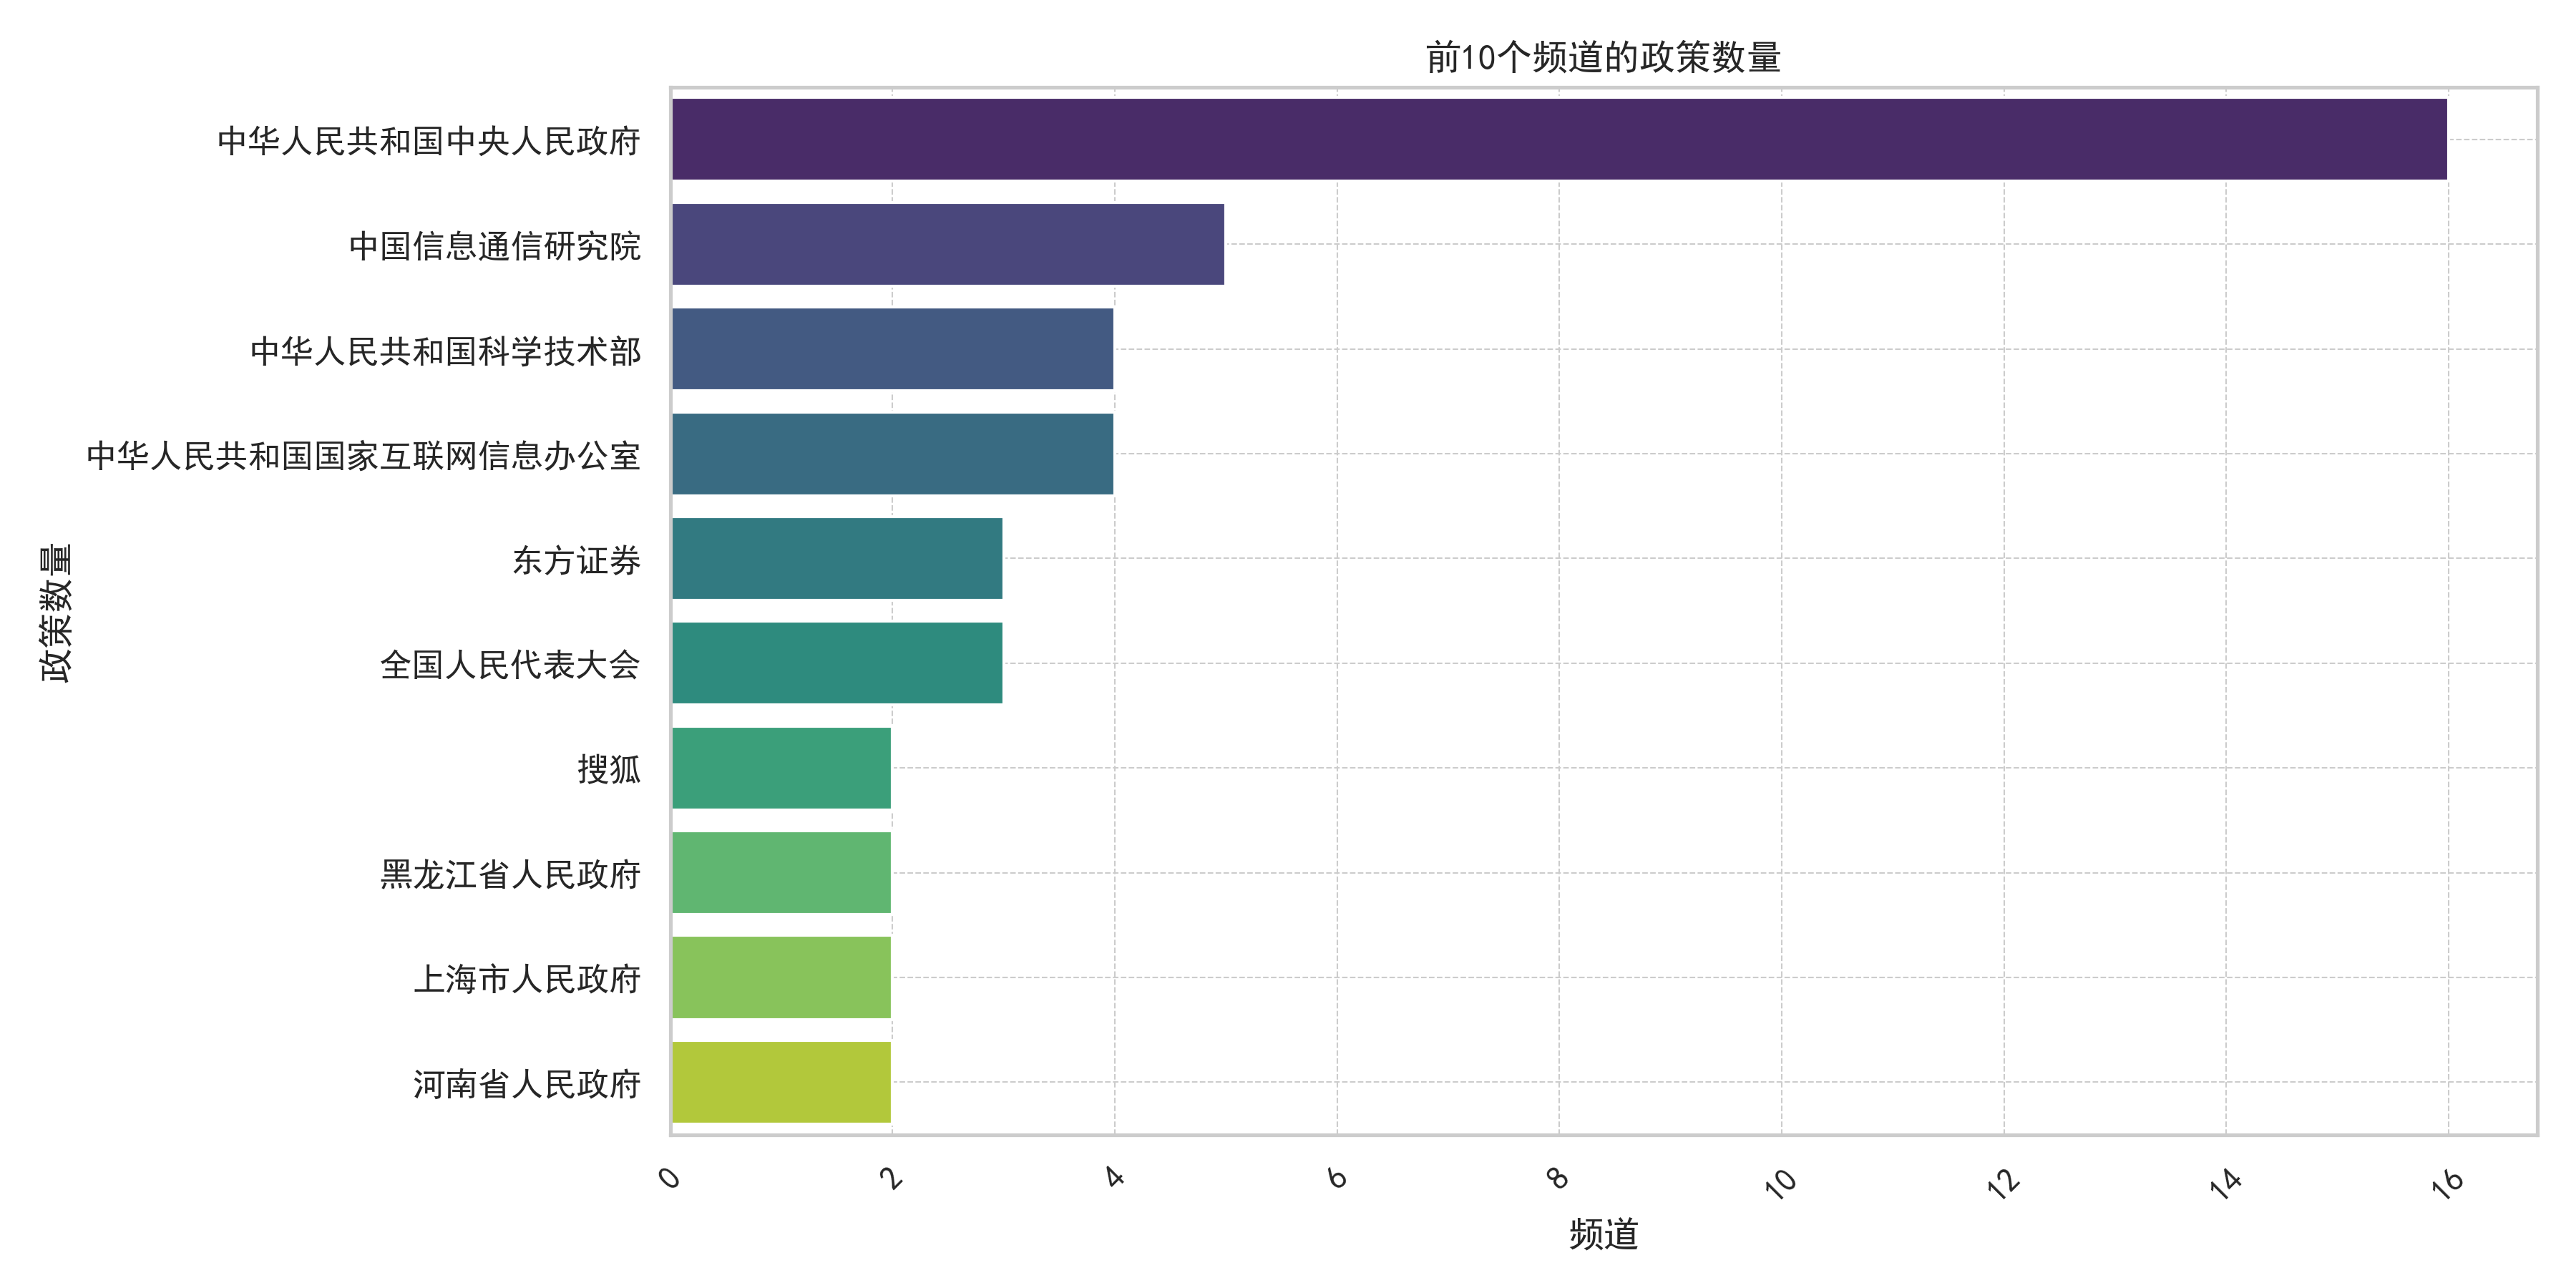
\includegraphics[width=1\textwidth]{images/top_10_channels_policy_count.png}
    \caption{政策文本数据集的前十个来源}
    \label{fig:top_10_channels_policy_count}
\end{figure}

本政策文本数据集的发布时间与内容长度分布如图\ref{fig:policy_pubtime_log_content_length}所示。数据集的时间范围为2010年到2025年。大部分政策集中在2020年之后,尤其是2021年到2023年之间,说明这段时间政策发布较为密集。内容长度主要集中在$10^3$到$10^4$之间。少量政策的内容长度较短或较长。在2010年和2011年有少量早期政策,某些年份(如2014年到2018年)几乎没有政策记录,可能是数据缺失或政策发布较少。随着时间推移,政策的数量逐渐增加。

\begin{figure}[H]
    \centering
    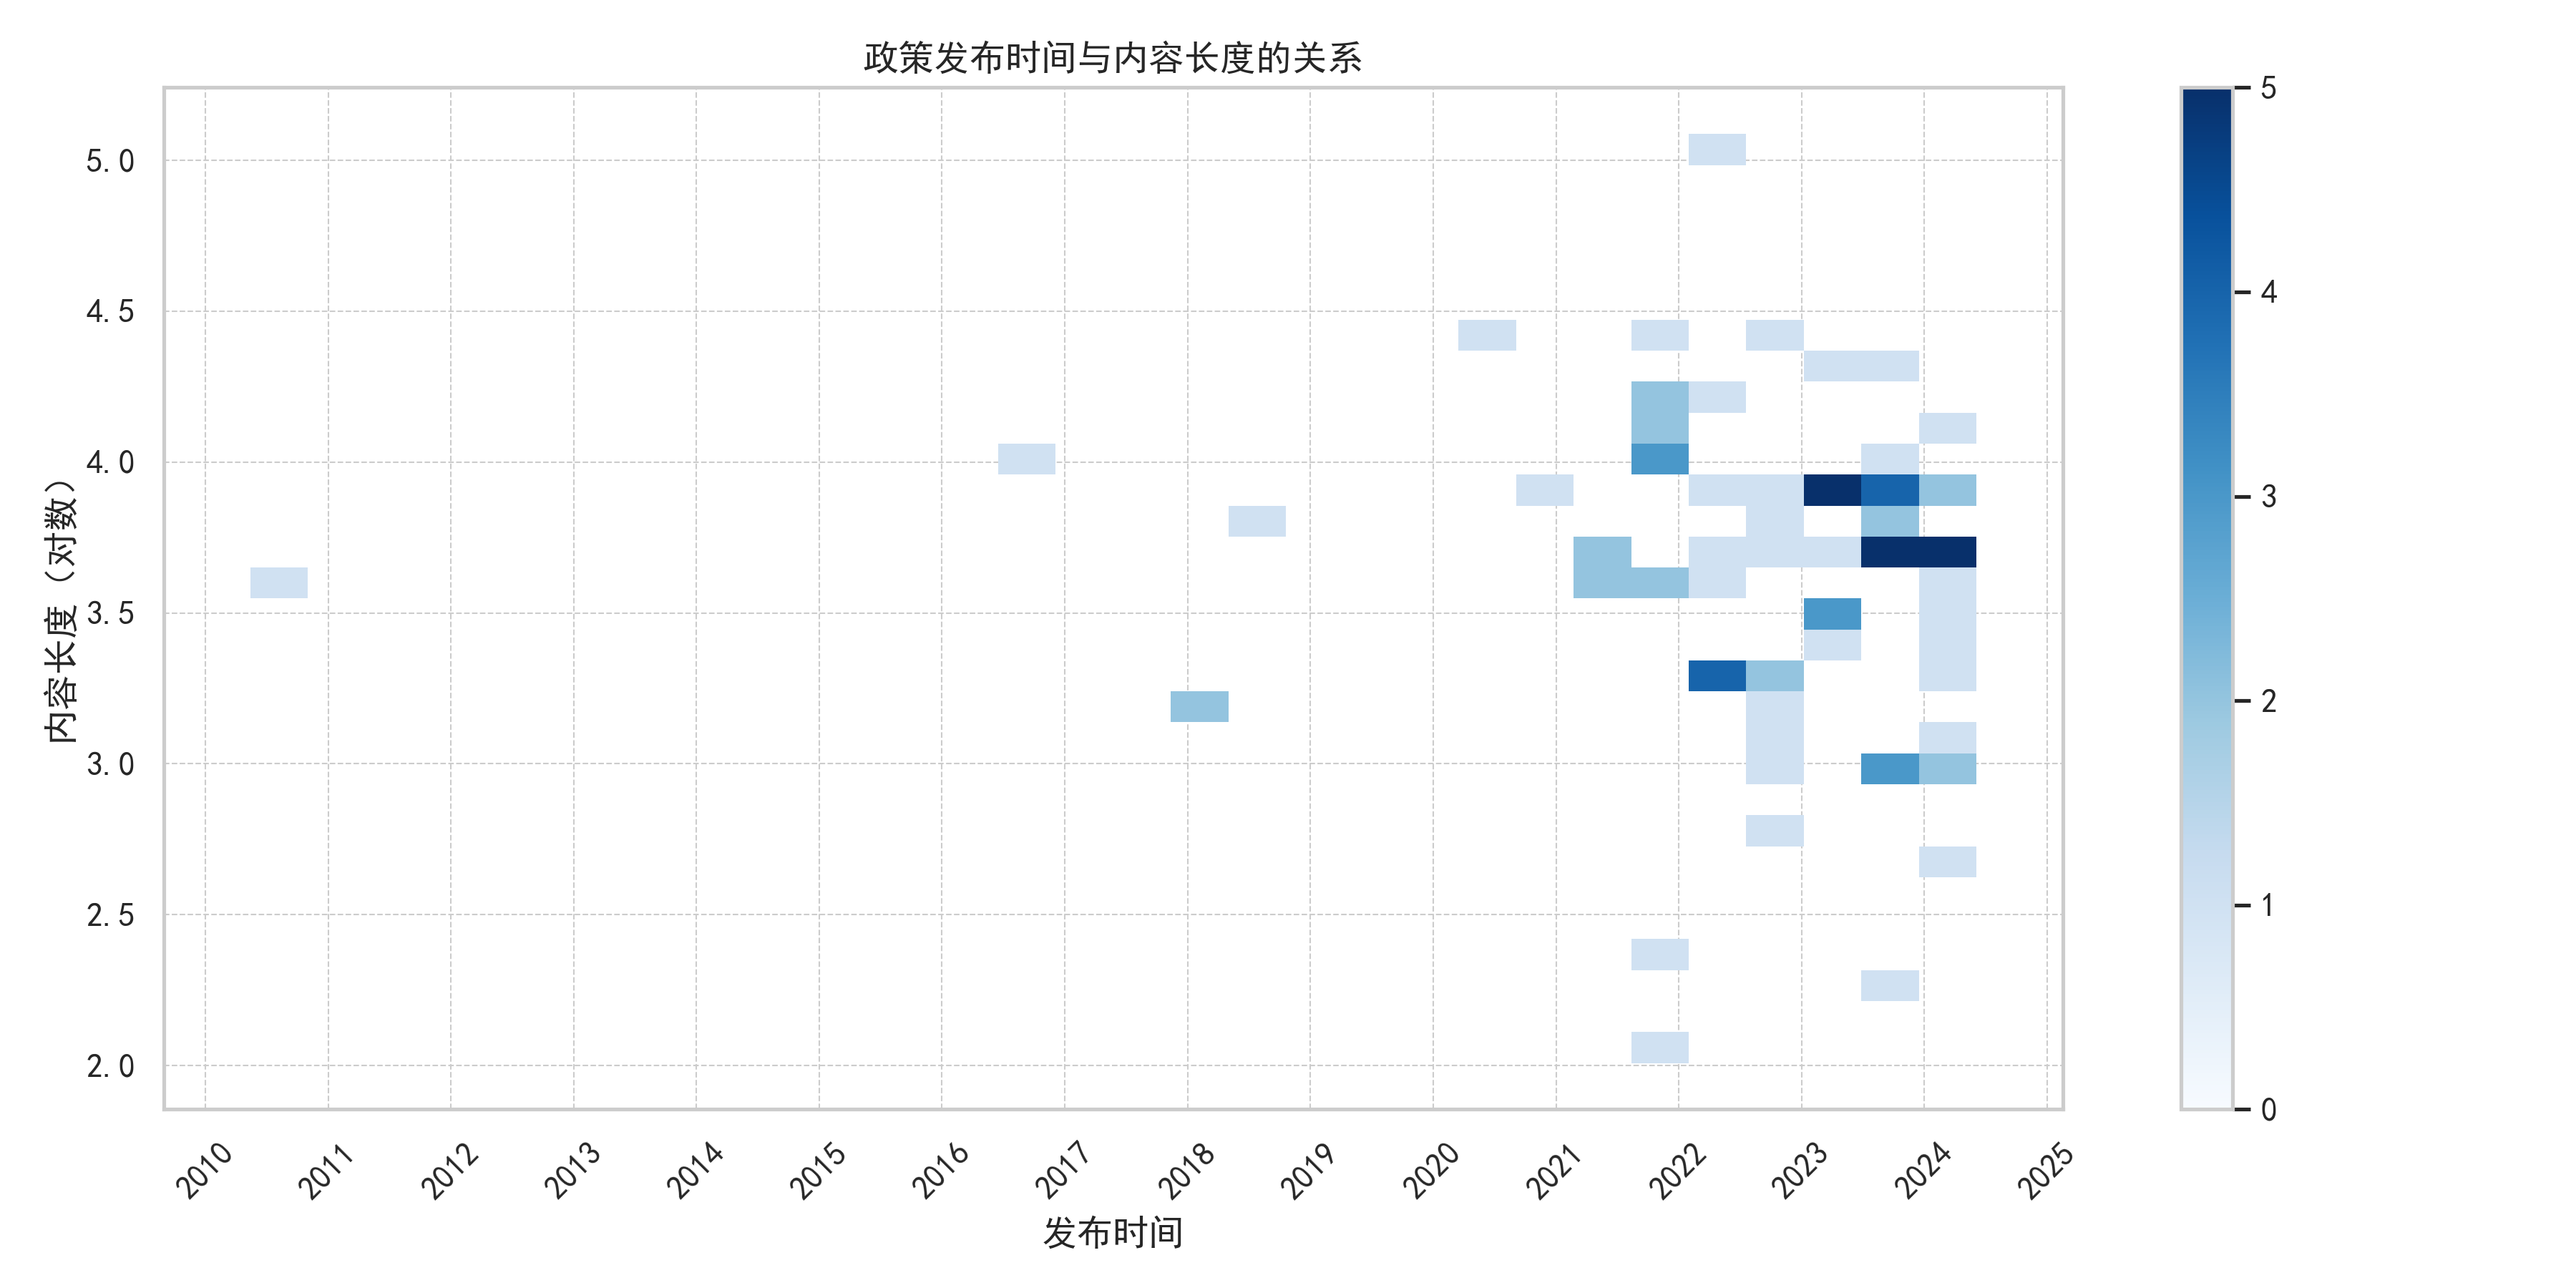
\includegraphics[width=1\textwidth]{images/policy_pubtime_log_content_length.png}
    \caption{政策文本数据集的发布时间与内容长度分布}
    \label{fig:policy_pubtime_log_content_length}
\end{figure}


最终构建的政策文本语料共计 99 篇文档,涵盖不同政策类别与区域来源,包括宏观经济、财政税收、乡村振兴、教育改革、公共卫生等多个细分领域。文本总句数为 19,335 句,文档平均句子数为195.3句,平均字符数9177.52字,总字符数达约90万汉字,句子平均长度为 64.83字/句,具备典型政策文风特征(长句、嵌套多、名词短语密集)。数据集描述性信息如表\ref{tab:policy_dataset_description}所示。

\begin{table}[H]
    \renewcommand{\arraystretch}{1}
    \centering
    \caption{政策文本数据集描述性信息}
    \label{tab:policy_dataset_description}
    \begin{tabular}{lcc}
        \toprule
        \textbf{指标} & \textbf{值} \\ 
        \midrule
        文档数量 & 99 \\
        总句子数 & 19335 \\
        平均句子数/文档 & 195.3 \\
        平均字符数/文档 & 9177.52 \\ 
        总字符数 & 900,000+ \\ 
        平均句子长度(字/句) & 64.83 \\
        \bottomrule
    \end{tabular}
\end{table}

\subsubsection{数据预处理}
在正式输入模型训练与评估之前,需对原始政策文本数据进行系统性预处理,以确保语料干净、结构统一,并充分提取粒度丰富的语言单元以用于编码器输入。
由于部分政策文本来自于扫描版文档或PDF转换结果,存在典型的OCR噪声,如断行错误、多余换行符、标点残缺、非正文符号嵌入等。我们对文本进行了如下处理:

将所有非段落边界的换行符(\textbackslash n)替换为空格,避免长句被错误截断;修复常见中英文混排标点错误(如“:”变为“:”),统一中文全角标点风格;移除低频率出现的非Unicode汉字字符、控制符(如\textbackslash x0c)、多余空格或乱码;清洗后文本结构更加规整,显著提升了后续“词级信息”提取的质量与鲁棒性。

政策类文本中,常包含表格信息、超链接、页脚编号、批注引用等非自然语言结构。这些信息对于模型训练而言往往是噪声,需予以剔除。本文采用基于正则表达式的规则方法进行清理,匹配带有明显网格、对齐线性结构的文本片段,如“|xxx|yyy|”或“——”连接的列名,并删除。去除所有形如 “http[s]”、“.com” 的 URL 链接;
利用常见模式(如“第x页”、“附件x”、“××年××号”)识别页脚、页码信息,并从段落中剥离;去除括号中的编号批注(如“(1)”、“[图1]”),并重构自然语言句式。

基于n-gram的分词策略在中文文本处理中存在一定局限性,这是因为其通过计算每两个字符中间的PMI(Pointwise Mutual Information)来确定n-gram片段的边界,可能导致切分出一些不符合中文语言习惯的片段,尤其是在处理多义词、成语或专有名词时。此外,n-gram方法在处理长文本时可能会产生大量的冗余片段,增加了模型的计算复杂度和内存消耗。并且,由于没有引入停用词过滤机制,可能会导致一些常见但对语义理解没有实际贡献的词被纳入模型训练中,从而影响模型的性能。

相比基于n-gram的策略,本文使用的HanLP提供了更语义驱动的中文分词工具,其基于神经网络词法分析模型,并支持自定义词典增强分词效果。使用 HanLP提供的api接口对清洗后的句子进行切词,去除停用词与其他不符合规则的词,统计词表中的词频,剔除低频词(出现次数小于10次)以减少噪声对模型训练的影响。最终构建的词表包含2662个词,覆盖了99.8\%的句子。

\subsubsection{微调数据集构建}
为评估改进后的中文文本编码器对上下文建模能力的增强效果,本文构建了一个适用于中文领域政策文本的$Next Sentence Prediction (NSP)$任务数据集。不同于英文NSP任务中基于自然段的句子抽取,中文文本中句子划分粒度模糊、标点使用灵活,因此我们结合句号(“。”)与逗号(“,”)进行多粒度分割,设计出更贴合中文语言结构的样本生成策略。

正样本的构建遵循“语义连续、上下文自然”的原则。我们首先使用HanLP对原始政策语料进行句子划分,按“中文句号(。)”作为分句边界,得到句子集合:
\begin{equation}
\mathcal{S} = \{s_1, s_2, \ldots, s_n\}
\end{equation}

对于每个句子我们利用“逗号”划分子句:
\begin{equation}
s_i = \{s_{i,1}', s_{i,2}', \ldots, s_{i,k}'\}
\end{equation}

将相邻的子句对 $(s_{i,k}, s_{i,k+1})$ 作为正样本对 $(s_i, s_{i+1})$,即:
\begin{equation}
(s_{i,k}, s_{i,k+1}) \in \mathcal{P}
\end{equation}

最终得到的正样本对数量为:
\begin{equation}
|\mathcal{P}| = 23374
\end{equation}

针对负样本,我们设计了两种生成策略,分别体现不同的训练目标与数据分布假设。

\textbf{方案一:}正负样本比例1:1,包含“句子顺序扰动”样本

该策略下,负样本数与正样本数相等,即:
\begin{equation}
|\mathcal{N}_1| = |\mathcal{P}| = 23374
\end{equation}

在构造负样本 $(s'_i, s'_j) \in \mathcal{N}_1$ 时,采用如下两类样本来源:

1. 顺序颠倒型(20\%):从正样本中选取20\%的句子对 $(s_i, s_{i+1})$,反转顺序构造 $(s_{i+1}, s_i)$;

2. 跨文档随机型(80\%):从整个语料库中随机选取两个不相邻句子 $(s'_i, s'_j)$,其中 $s'_i$ 和 $s'_j$ 可来自不同文章或不同段落,确保语义无关。

该策略优点在于正负样本数量平衡,有助于训练模型识别语义连贯性,并关注句子顺序是否合理。
我们将该方案的数据集称为PolicySM-1(Policy Sentence Matching 1)。然而,由于来自不同文章的句子有概率在语义上具有相似性,如两篇介绍地区“数据治理政策”的文章可能都提到“数据治理”这一概念,因此该方案的负样本可能会引入一些噪声,导致模型的训练结果无法很好地反映句子间的真实关系。为此,我们引入了第二个数据集方案。

\vspace{2em} % 添加空行

\textbf{方案二:}正负样本比例1:5,基于篇内语义混淆构造

在第二种策略中,我们设计更复杂的负样本:从同一篇文章中抽取相隔2至5句话的句子对,并在其内部使用逗号划分子句以混淆语义边界。即,对于句子序列 $\{s_i\}$,构造如下样本对:

\begin{equation}
(s_{i,k}, s_{j,l}) \quad \text{其中} \quad j = i + \delta,\quad \delta \in \{2, 3, 4, 5\}
\end{equation}

其中 $s_{i,k}$ 和 $s_{j,l}$ 分别为句子 $s_i$ 和 $s_j$ 中用逗号划分出的任一子句。最终采样形成:

\begin{equation}
|\mathcal{N}_2| = 5 \times |\mathcal{P}| = 116870
\end{equation}

该方案的设计意图在于强化模型对篇内局部干扰与语义跳跃的辨别能力,提升编码器对更细粒度上下文关系的建模能力。尤其是在RAG任务中,模型需要能够区分相关与不相关的句子对,以便在检索阶段准确匹配问题与答案。而同一篇文章中相隔较远的句子往往比起随机选取句子更能体现语义上的差异。而更多的负样本数量也有助于模型学习到更丰富的语义信息,避免过拟合。因此,方案二的负样本构造更贴近实际应用场景,能够有效提升模型的泛化能力。我们将方案二的数据集称为PolicySM-2(Policy Sentence Matching 2)。

我们分别采用方案一与方案二构建了两个NSP训练数据集,分布如表 \ref{tab:nsp_samples} 所示。

\begin{table}[H]
    \centering
    \caption{NSP任务样本分布}
    \begin{tabular}{lcccc}
        \toprule
        数据集 & 正样本数 & 负样本数 & 正负比例 & 总样本数 \\
        \midrule
        PolicySM-1 & 23374 & 23374 & 1:1 & 46748 \\
        PolicySM-2 & 23374 & 116870 & 1:5 & 140244 \\
        \bottomrule
    \end{tabular}
    \label{tab:nsp_samples}
\end{table}

在后续实验部分,我们将分别基于两种方案训练NSP任务模型,并评估不同样本构造策略对文本编码器语义理解能力的影响。

\subsubsection{骨干模型}
有关于模型的具体实现,本文基于 $Hugging Face$ 的 Transformers 库,使用了 $ZEN-pretrain-base$ 模型和 $bge-base-zh-v1.5$ 模型。前者是基于 BERT 的中文预训练模型,拥有预训练的字符嵌入与词嵌入参数。后者是 BAAI 提出的中文通用嵌入模型,主要用于RAG任务中的文本嵌入生成。对$bge$模型的处理如图\ref{fig:model_merge}所示,我们将 $bge-base-zh-v1.5$ 的主体 BERT 部分参数提取出来作为骨干字符嵌入模型,其余的参数则使用 $ZEN-pretrain-base$ 模型进行初始化。微调过的 $bge-base-zh-v1.5$ 模型将被用于后续的RAG系统中。

\begin{figure}[H]
    \centering
    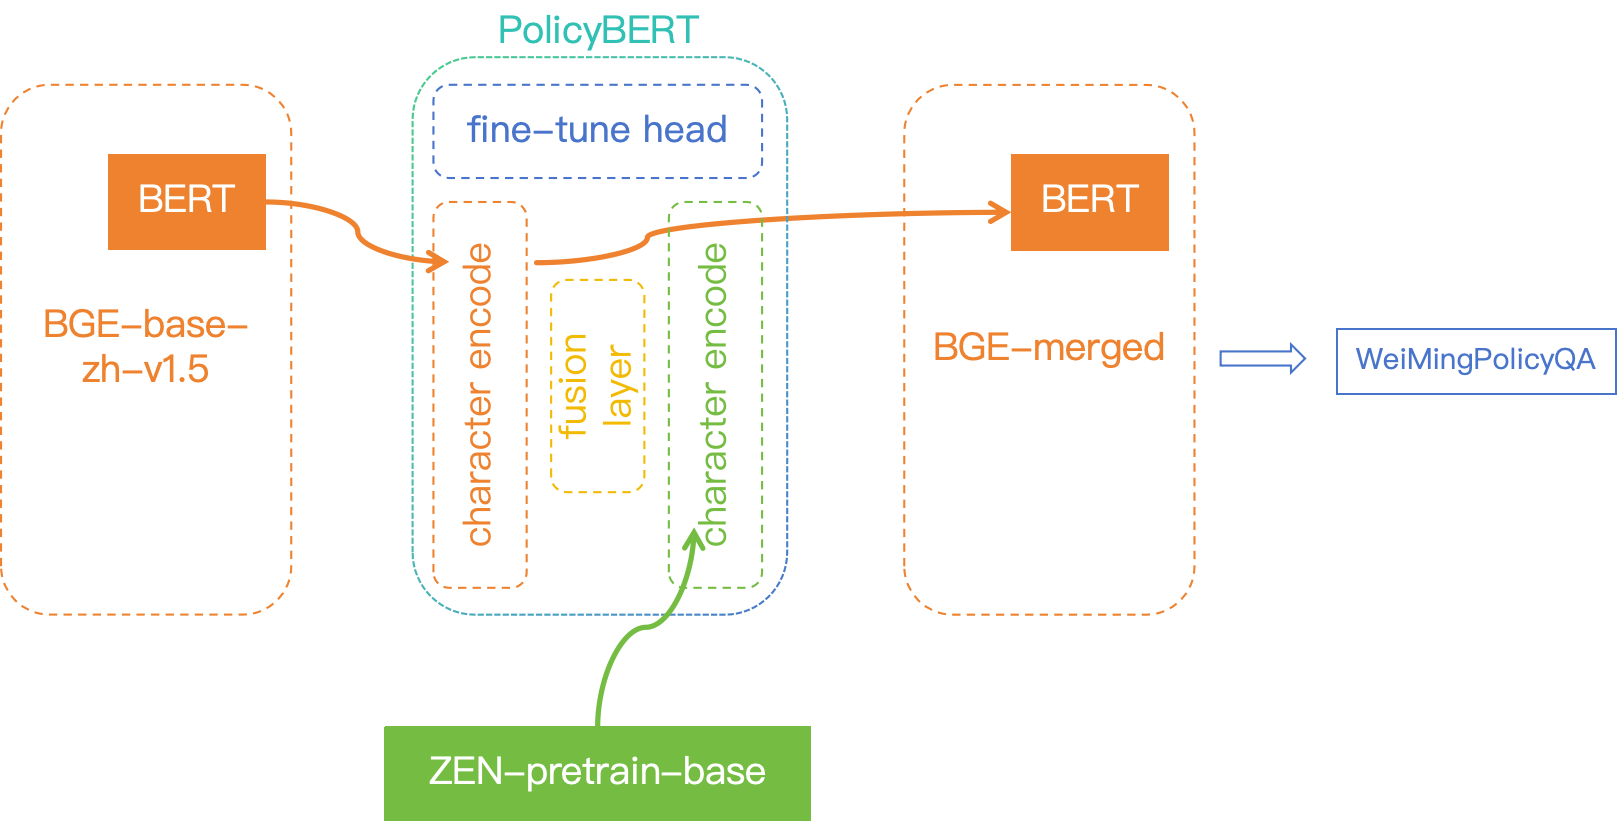
\includegraphics[width=0.8\textwidth]{images/model_merge.png}
    \caption{对bge模型的处理,将其主体BERT部分参数提取出来作为骨干字符嵌入模型,其余的参数使用ZEN预训练模型进行初始化,微调过的bge模型将被用于后续的RAG系统中。}
    \label{fig:model_merge}
\end{figure}


\subsubsection{训练配置}
实验在一台高性能GPU服务器上进行,配置如下:

\begin{itemize}
    \item GPU:NVIDIA RTX 4090 × 1,显存 24 GB
    \item CPU:20 核 Intel Xeon 处理器
    \item 内存:80 GB
    \item 工作空间:50 GB SSD 存储用于中间缓存与模型权重
    \item 框架:PyTorch 2.0,python 3.8,cuda 11.8
\end{itemize}

该配置确保了在处理大规模预训练模型和多层融合机制时具备稳定的训练性能和内存调度能力。

\subsection{实验结果}
\subsubsection{公开数据集}
首先,我们将在公开数据集上进行实验,与现有的NLP领域文本编码器进行对比。包括 BERT-wwm, ERNIE 1.0,ERNIE 2.0, NEZHA 和 ZEN。我们使用了 ZEN 的预训练模型作为基线模型进行微调。我们使用了不同的融合方法(门控机制、多头注意力机制)进行对比。由于缺少大规模预训练语料,我们无法在公开数据集上应用Hanlp分词,也无法进行对基线模型的预训练。因此我们在公开数据集上仅测试了不同融合方法与n-gram表示的效果。

我们在以下任务上进行了评估:
\begin{itemize}
    \item \textbf{中文分词(CWS):} 使用 SIGHAN2005 中文分词评测(Emerson, 2005)\cite{emerson-2005-second}中的 MSR 数据集。
    \item \textbf{词性标注(POS):} 使用 CTB5 数据集(Xue 等, 2005)\cite{10.1017/S135132490400364X},并采用标准数据划分。
    \item \textbf{命名实体识别(NER):} 使用国际中文语言处理评测 (Bakeoff 2006)\cite{levow-2006-third} 中的 MSRA 数据集。
    \item \textbf{文档分类(DC):} 使用 THUCNews 数据集(Sun 等, 2016)\cite{sun2016thuctc},该数据集来源于新浪新闻,包含 10 个类别,类别分布均匀。
    \item \textbf{情感分析(SA):} 使用 ChnSentiCorp(CSC)数据集\cite{yfwt-wr77-20},该数据集包含来自图书、计算机和酒店三个领域的 12,000 篇文档。
    \item \textbf{句子对匹配(SPM):}使用 LCQMC 数据集(Liu 等, 2018)\cite{liu-etal-2018-lcqmc},该数据集中的每一个样本都是一个句子对,和一个标签,表示这两个句子是否语义相似。
\end{itemize}

各个任务的数据集划分和数据集内句子/文档数量如表 \ref{tab:public_datasets} :

\begin{table}[H]
    % 设置行高
    \renewcommand{\arraystretch}{1}
    \centering
    \caption{公开数据集上各个任务的数据集划分,包括训练集和测试集的大小}
    \begin{tabular}{l|cccccc}
        \toprule
        \textbf{Task} & CWS & POS & NER & DC & SA & SPM\\
        \midrule
        \textbf{Dataset} & MSR & CTB5 & MSRA & THUCNews & CSC & LCQMC\\
        \midrule
        \textbf{Train} & 87K & 18K & 45K & 50K & 10K & 239K \\
        \textbf{Test} & 4K & 1K & 3K & 10K & 1K & 13K \\
        \bottomrule
    \end{tabular}
    \label{tab:public_datasets}
\end{table}

表 \ref{tab:public_results} 展示了不同模型在公开数据集上的F1值对比结果,可以看出,PolicyBERT在多个任务上均表现出色,尤其是在中文分词(CWS)和词性标注(POS)任务中,分别达到了0.9816和0.9716的F1值,显著优于两个基线模型(BERT和ZEN)。
此外,在句子对匹配(SPM)任务中,PolicyBERT的多头注意力机制(attn)和门控机制(gate)融合方法分别达到了0.9016和0.8997的F1值,分别为最高和次高的结果,远超过其他所有模型,表明其在捕捉上下文语义关系方面具有明显优势。
虽然在命名实体识别(NER)和文档分类(DC)任务中,PolicyBERT的表现略逊于一些大模型(如ERNIE 2.0),但其表现仍然具有竞争力,且在NER任务中,PolicyBERT的注意力机制融合方法(attn)达到了0.9437的F1值,为次高的结果,显示出其在处理复杂语义关系时的潜力。在文档分类(DC)任务中,PolicyBERT的表现相对较弱,F1值为0.9655,略低于一些大模型(如ERNIE 2.0和NEZHA),但仍然保持在较高水平,显示出其在处理长文本时的稳定性和可靠性。
在情感分析(SA)任务中,PolicyBERT的表现也相对较好,达到了0.9475的F1值,表明其在处理情感倾向性文本时具有一定的优势。总体而言,PolicyBERT在多个任务上均展现出良好的性能,尤其是在中文分词和句子对匹配任务中,显示出其在上下文建模和语义理解方面的优势。

\begin{table}[H]
    \renewcommand{\arraystretch}{1}
    \centering
    \caption{公开数据集上不同模型的f1值对比,其中$B$表示基线模型,$L$表示大模型,attn和gate分别表示多头注意力机制和门控机制融合方法。加粗和下划线分别表示在同一列中最好的和次好的结果。}
    \begin{tabular}{lcccccc}
        \toprule
        \textbf{Model\textbackslash Task} & CWS & POS & NER & DC & SA & SPM \\
        \midrule
        BERT      & 0.9720 & 0.9543 & 0.9312 & 0.9671 & 0.9410 & 0.8513\\
        \midrule
        BERT-wwm     & - & - & \textbf{0.9510} & \textbf{0.9760} & 0.9500 & 0.8680\\
        ERNIE 1.0    & - & - & 0.9510 & \underline{0.9730} & 0.9540 & 0.8740 \\
        ERNIE 2.0(B) & - & - & -      & -      & 0.9550 & 0.8790\\
        NEZHA(B)     & - & - & -      & -      & 0.9517 & 0.8741\\
        NEZHA-wwm(B) & - & - & -      & -      & \underline{0.9584} & 0.8710\\
        \midrule
        ERNIE 2.0(L) & - & - & -      & -      & 0.9580 & 0.8790\\
        NEZHA(L)     & - & - & -      & -      & 0.9583 & 0.8720\\
        NEZHA-wwm(L) & - & - & -      & -      & \textbf{0.9600} & 0.8794\\
        \midrule
        ZEN       & 0.9789 & 0.9582 & 0.9324 & 0.9687 & 0.9442 & 0.8527\\
        \midrule
        $PolicyBERT_{attn}$ & \underline{0.9812} & \underline{0.9711} & \underline{0.9437} & 0.9651 & 0.9441 & \textbf{0.9016}\\
        $PolicyBERT_{gate}$ & \textbf{0.9816} & \textbf{0.9716} & 0.9422 & 0.9655 & 0.9475 & \underline{0.8997}\\ 
        \bottomrule
    \end{tabular}
    \label{tab:public_results} 
\end{table}

\subsubsection{PolicySM-1}
我们在PolicySM-1数据集上测试了不同融合方法与Hanlp分词的效果。在这部分实验中,我们仅使用ZEN-pretrain-base模型作为基础模型,使用了不同的融合方法(门控机制、多头注意力机制)与原始论文中直接相加进行对比。并对比了使用Hanlp分词与使用n-gram表示的效果。

预训练和下游任务的训练超参数分别如表 \ref{tab:pretrain_hyperparameters_1} 和表 \ref{tab:seqlevel_hyperparameters_1} 所示。


\begin{table}[H]
    \renewcommand{\arraystretch}{1}
    \centering
    \caption{PolicySM-1预训练超参数}
    \begin{tabular}{lcccc}
        \toprule
        \textbf{参数名称} & \textbf{参数取值} & \textbf{描述} \\
        \midrule
        \texttt{epochs} & 3 & 总训练轮数 \\ 
        \texttt{train\_batch\_size} & 32 & 训练批量 \\
        \texttt{learning\_rate} & 3e-5 & 初始学习率 \\ 
        \texttt{warmup\_proportion} & 0.9 & 学习率预热比例 \\ 
        \bottomrule
    \end{tabular}
    \label{tab:pretrain_hyperparameters_1}
\end{table}

\begin{table}[H]
    \renewcommand{\arraystretch}{1}
    \centering
    \caption{PolicySM-1下游任务超参数}
    \begin{tabular}{lcccc}
        \toprule
        \textbf{参数名称} & \textbf{参数取值} & \textbf{描述} \\ 
        \midrule
        \texttt{max\_seq\_length} & 128 & 最大输入长度\\ 
        \texttt{train\_batch\_size} & 32 & 训练批量 \\ 
        \texttt{eval\_batch\_size} & 8 & 评估的批量大小 \\
        \texttt{learning\_rate} & 5e-5 & 初始学习率 \\
        \texttt{num\_train\_epochs} & 3 & 总训练轮数 \\ 
        \texttt{warmup\_proportion} & 0.9 & 学习率预热比例 \\
        \bottomrule
    \end{tabular}
    \label{tab:seqlevel_hyperparameters_1}
\end{table}

实验结果由表 \ref{tab:fusion_results_1} 所示。可以看到,使用Hanlp分词的模型在所有融合方法中表现最好,达到了0.9132的准确率。使用n-gram表示的模型在Attention-based Fusion下也取得了不错的效果,达到了0.9121的准确率。这意味着,使用Hanlp分词的模型在处理中文政策文本时,能够更好地捕捉到词语之间的关系和上下文信息,从而提高了模型的性能。而两种融合方法与原始论文中直接相加的效果相比,均有了显著提升,说明引入门控机制和多头注意力机制能够有效增强模型对中文政策文本的建模能力。

\begin{table}[ht]
    \renewcommand{\arraystretch}{1}
    \centering
    \caption{PolicySM-1下游任务结果}
    \begin{tabular}{lcc}
    \hline
    \textbf{融合方法} & \textbf{分词方法} & \textbf{准确率} \\
    \hline
    None                   & n-gram                   & 0.8867 \\
    Gated Fusion           & n-gram                  & 0.8959 \\
    Attention-based Fusion   & n-gram                 & \textbf{0.9121}\\
    \hline
    None                   & Hanlp                       & 0.9035 \\
    Gated Fusion           & Hanlp                       & 0.8981 \\
    Attention-based Fusion   & Hanlp                     & \textbf{0.9132} \\
    \hline
    \end{tabular}
    \label{tab:fusion_results_1}
\end{table}

\newpage

\subsubsection{PolicySM-2}
我们在PolicySM-1数据集上同时测试了两个模型(ZEN-pretrain-base和bge-base-zh-v1.5)在不同融合方法下的效果。预训练和下游任务的训练超参数分别如表 \ref{tab:pretrain_hyperparameters_2} 和表 \ref{tab:seqlevel_hyperparameters_2} 所示。由于先前的实验已经验证了使用Hanlp分词的模型在所有融合方法中表现最好,因此我们在这部分实验中仅使用了Hanlp分词。

\begin{table}[H]
    \renewcommand{\arraystretch}{1}
    \centering
    \caption{PolicySM-2预训练超参数}
    \begin{tabular}{lcccc}
        \toprule
        \textbf{参数名称} & \textbf{参数取值} & \textbf{描述} \\
        \midrule
        \texttt{epochs} & 5 & 总训练轮数 \\ 
        \texttt{train\_batch\_size} & 32 & 训练批量 \\
        \texttt{learning\_rate} & 3e-5 & 初始学习率 \\ 
        \texttt{warmup\_proportion} & 0.9 & 学习率预热比例 \\ 
        \bottomrule
    \end{tabular}
    \label{tab:pretrain_hyperparameters_2}
\end{table}

\begin{table}[H]
    \renewcommand{\arraystretch}{1}
    \centering
    \caption{PolicySM-2下游任务超参数}
    \begin{tabular}{lcccc}
        \toprule
        \textbf{参数名称} & \textbf{参数取值} & \textbf{描述} \\ 
        \midrule
        \texttt{max\_seq\_length} & 128 & 最大输入长度\\ 
        \texttt{train\_batch\_size} & 32 & 训练批量 \\ 
        \texttt{eval\_batch\_size} & 8 & 评估的批量大小 \\
        \texttt{learning\_rate} & 5e-5 & 初始学习率 \\
        \texttt{num\_train\_epochs} & 3 & 总训练轮数 \\ 
        \texttt{warmup\_proportion} & 0.9 & 学习率预热比例 \\
        \bottomrule
    \end{tabular}
    \label{tab:seqlevel_hyperparameters_2}
\end{table}

实验结果由表 \ref{tab:pretrain-results} 和表 \ref{tab:nsp-results} 所示。我们可以看到,在预训练任务中,使用了门控机制和多头注意力机制的模型在MLM Loss、MLM 准确率和困惑度上均有显著提升,尤其是使用多头注意力机制的模型在所有指标上均达到了最优值。这表明,融合式中文编码模型能够有效地捕捉到字符和词之间的关系,从而提高了模型的性能。

而在下游任务中,使用了门控机制和多头注意力机制的模型在NSP准确率上也有显著提升,尤其是使用多头注意力机制的模型在NSP准确率上达到了最优值。这表明,融合式中文编码模型能够有效地捕捉到上下文信息,从而提高了模型的性能。

\begin{table}[htbp]
    \renewcommand{\arraystretch}{1}
    \centering
    \caption{PolicySM-2预训练结果}
    \begin{tabular}{llccc}
      \toprule
      骨干模型 & 融合方法 & MLM Loss & MLM acc & 困惑度 \\
      \midrule
      \multirow{3}{*}{BGE}
        & none & 1.0151 & 0.7837 & 2.76 \\
        & gate & 0.9763 & 0.7924 & 2.65 \\
        & attn & \textbf{0.9218} & \textbf{0.8029} & \textbf{2.51} \\
      \midrule
      \multirow{3}{*}{ZEN}
        & none & 0.9064 & 0.8036 & 2.48 \\
        & gate & 0.9332 & 0.7995 & 2.54 \\
        & attn & \textbf{0.8952} & \textbf{0.8059} & \textbf{2.45} \\
      \bottomrule
    \end{tabular}
    \label{tab:pretrain-results}
  \end{table}
  
  \begin{table}[htbp]
    \renewcommand{\arraystretch}{1}
    \centering
    \caption{PolicySM-2下游任务结果}
    \begin{tabular}{llc}
      \toprule
      骨干模型 & 融合方法 & NSP acc \\
      \midrule
      \multirow{3}{*}{BGE}
        & none & 0.9236 \\
        & gate & \textbf{0.9311} \\
        & attn & 0.9272 \\
      \midrule
      \multirow{3}{*}{ZEN}
        & none & 0.9260 \\
        & gate & \textbf{0.9325} \\
        & attn & 0.9274 \\
      \bottomrule
    \end{tabular}
    \label{tab:nsp-results}
  \end{table}

\newpage
\section{未名问政}
\begin{figure}[H]
    \centering
    
\includegraphics[width=0.8\textwidth]{./images/WeiMingPolicyLogo.png}
    \caption{未名问政Logo}
    \label{fig:WeiMingLogo}
\end{figure}

\subsection{系统架构}

前文通过在政策文本语料上的微调,显著提升了 $bge\text{-}base\text{-}zh\text{-}v1.5$ 模型在子领域内对中文语义的理解与表达能力。在此基础上,本文进一步构建了一个基于检索增强生成(Retrieval-Augmented Generation, RAG)机制的智能问答系统,命名为“未名问政”,以提供高效、精准的政策解读与咨询服务,帮助用户快速理解并获取所需政策信息。该系统采用了 Langchain-Chatchat 架构作为整体框架,在保障系统模块化、可扩展性的同时,方便快速集成主流语言模型与检索引擎。系统整体由三部分组成:检索模块、生成模块,以及一个轻量级的融合控制层,形成了完整的“查询—检索—生成—响应”工作链条。

在检索模块方面,系统使用了基于 PolicyBERT 架构并经过领域微调的 $bge\text{-}base\text{-}\\zh\text{-}v1.5$ 模型作为中文文本编码器。为进一步融合通用语义能力与子领域知识,本文将微调后的参数与原始模型部分参数拼接,构建了 $bge\text{-}base\text{-}zh\text{-}v1.5\text{-}merge$ 模型。具体流程为:首先对政策语料进行分段预处理(每段限制在750字以内),随后将其编码为固定维度的向量,存入本地 Faiss 向量数据库中。在用户输入查询后,系统会将查询文本同样编码为向量,并通过相似度检索选出 top‑k 个最相关的政策片段,作为后续生成模块的上下文支持。

在生成模块中,系统部署了通过 Ollama 实现本地化的 $Qwen2.5:7b$ 大语言模型。该模型具备长上下文处理能力与良好的中文语义生成效果,能够结合检索到的文本片段和用户原始问题,通过预设提示模板(Prompt)完成专业、连贯的答案生成过程。生成模块将检索模块输出的多个相关片段与查询拼接,并输入至 $Qwen2.5:7b$,最终输出针对性强、逻辑清晰的回答内容或政策摘要。

综上,本文构建的“未名问政”系统在本地硬件(RTX 4060 8GB 显存)上完成了从文本检索到问答生成的全流程部署,充分融合了 $bge\text{-}base\text{-}zh\text{-}v1.5\text{-}merge$ 的检索能力与 $Qwen2.5:7b$ 的生成优势,依托 Langchain-Chatchat 架构实现了高度模块化与可配置的中文 RAG 系统。该系统具备部署灵活、响应快速、扩展便捷等特点,尤其适用于政务智能问答、政策知识库构建与自动解读等典型场景。

\subsection{系统演示}

\subsubsection{系统部署}
未名问政RAG系统的部署过程相对简单,用户只需在本地安装必要的依赖库,并下载预训练模型与知识库数据。系统支持多种操作系统环境,包括Windows、Linux和MacOS。用户可根据需求选择合适的运行环境,并通过命令行界面启动系统。系统的运行效率较高,能够在普通个人电脑上实现快速响应。本次部署配置如下:
\begin{itemize}
    \item 操作系统:Windows 10
    \item CPU:Intel Core i9-14900HX
    \item 内存:32 GB
    \item 显卡:NVIDIA GeForce RTX 4060 8GB
    \item Python版本:3.9.6
\end{itemize}

部署前应提前配置Ollama环境,可于\href{https://ollama.com/}{\underline{Ollama官网}}下载Ollama,并通过以下代码部署千问模型(Qwen2.5:7b)和微调过的 $bge\text{-}base\text{-}zh\text{-}v1.5$ 模型。具体步骤如下:
\begin{itemize}
    \item 下载模型:在终端中运行以下命令,下载千问模型(Qwen2.5:7b):
    \begin{lstlisting}[language=bash]
        ollama pull qwen2.5:7b
    \end{lstlisting}
    \item 部署微调过的 $bge\text{-}base\text{-}zh\text{-}v1.5$ 模型:
    \begin{lstlisting}[language=bash]
        ollama add bge-base-zh-v1.5 path/to/your/model
    \end{lstlisting}
    \item 启动Ollama:在终端中运行以下命令,启动Ollama服务并保持运行:
    \begin{lstlisting}[language=bash]
        ollama serve
    \end{lstlisting}
\end{itemize}


使用代码将\href{https://github.com/PuHT4213/WeiMingPolicyRAG}{\underline{未名问政系统}}克隆到本地:
\begin{lstlisting}[language=bash]
    git clone https://github.com/PuHT4213/WeiMingPolicyRAG.git
    cd WeiMingPolicyRAG/lib/chatchat-server
\end{lstlisting}

创建虚拟环境,并安装必要的依赖库:
\begin{lstlisting}[language=bash]
    python3.9 -m venv weimingpolicyrag
    source weimingpolicyrag/bin/activate # Linux/MacOS
    weimingpolicyrag\Scripts\activate # Windows
    pip install -e .
\end{lstlisting}

确保政策文件在目录 \texttt{./libs/chatchat-server/chatchat/data/knowledge\_\\base/WeiMingPolicies/content}下,然后运行以下命令初始化并启动系统:
\begin{lstlisting}[language=bash]
    chatchat kb -r
    chatchat start -a
\end{lstlisting}

出现以下日志以及图\ref{fig:home_page}所示的界面后,表示系统已成功启动并运行。用户可在浏览器中访问并进行交互。
\begin{lstlisting}[language=bash]
    -----------------------------------------------------------
    知识库名称      :WeiMingPolicies
    知识库类型      :faiss
    向量模型:      :bge-large-zh-v1.5
    知识库路径      :path/to/your/knowledge_base
    文件总数量      :99
    入库文件数      :99
    知识条目数      :740
    用时            :0:02:29.701002
    -----------------------------------------------------------
    
    总计用时        :0:02:33.414425
\end{lstlisting} 

\subsubsection{RAG对话}
如图\ref{fig:home_page}所示,未名问政RAG系统的主界面简洁直观,当前版本为 \texttt{1.0.0.1}。界面左侧设有功能导航栏,用户可在“多功能对话”、“RAG 对话”与“知识库管理”等主要模块间进行切换。在“RAG 对话”模式下,用户可以根据具体需求,自定义相关配置参数。首先,用户可通过下拉菜单选择对话模式,目前支持“知识库问答”;随后可选择已加载的知识库,以支持特定领域的问答服务。进一步地,系统允许用户设置历史对话轮数(默认为3轮)、匹配知识条数(默认为5条),以及知识匹配的最低分数阈值(以滑动条形式设置,范围为 \texttt{0.00} 至 \texttt{2.00},默认值为 \texttt{0.50}),SCORE越小,相关度越高,取到2相当于不筛选。此外,用户还可以勾选“仅返回检索结果”选项,以查看未融合生成的原始检索片段。界面右侧为空白对话窗口区域,用于展示系统响应内容。底部提供输入框,支持多轮对话交互,用户输入内容后可按 \texttt{Shift+Enter} 执行提交,界面整体设计清晰高效,便于快速部署和应用。
\begin{figure}[H]
    \centering
    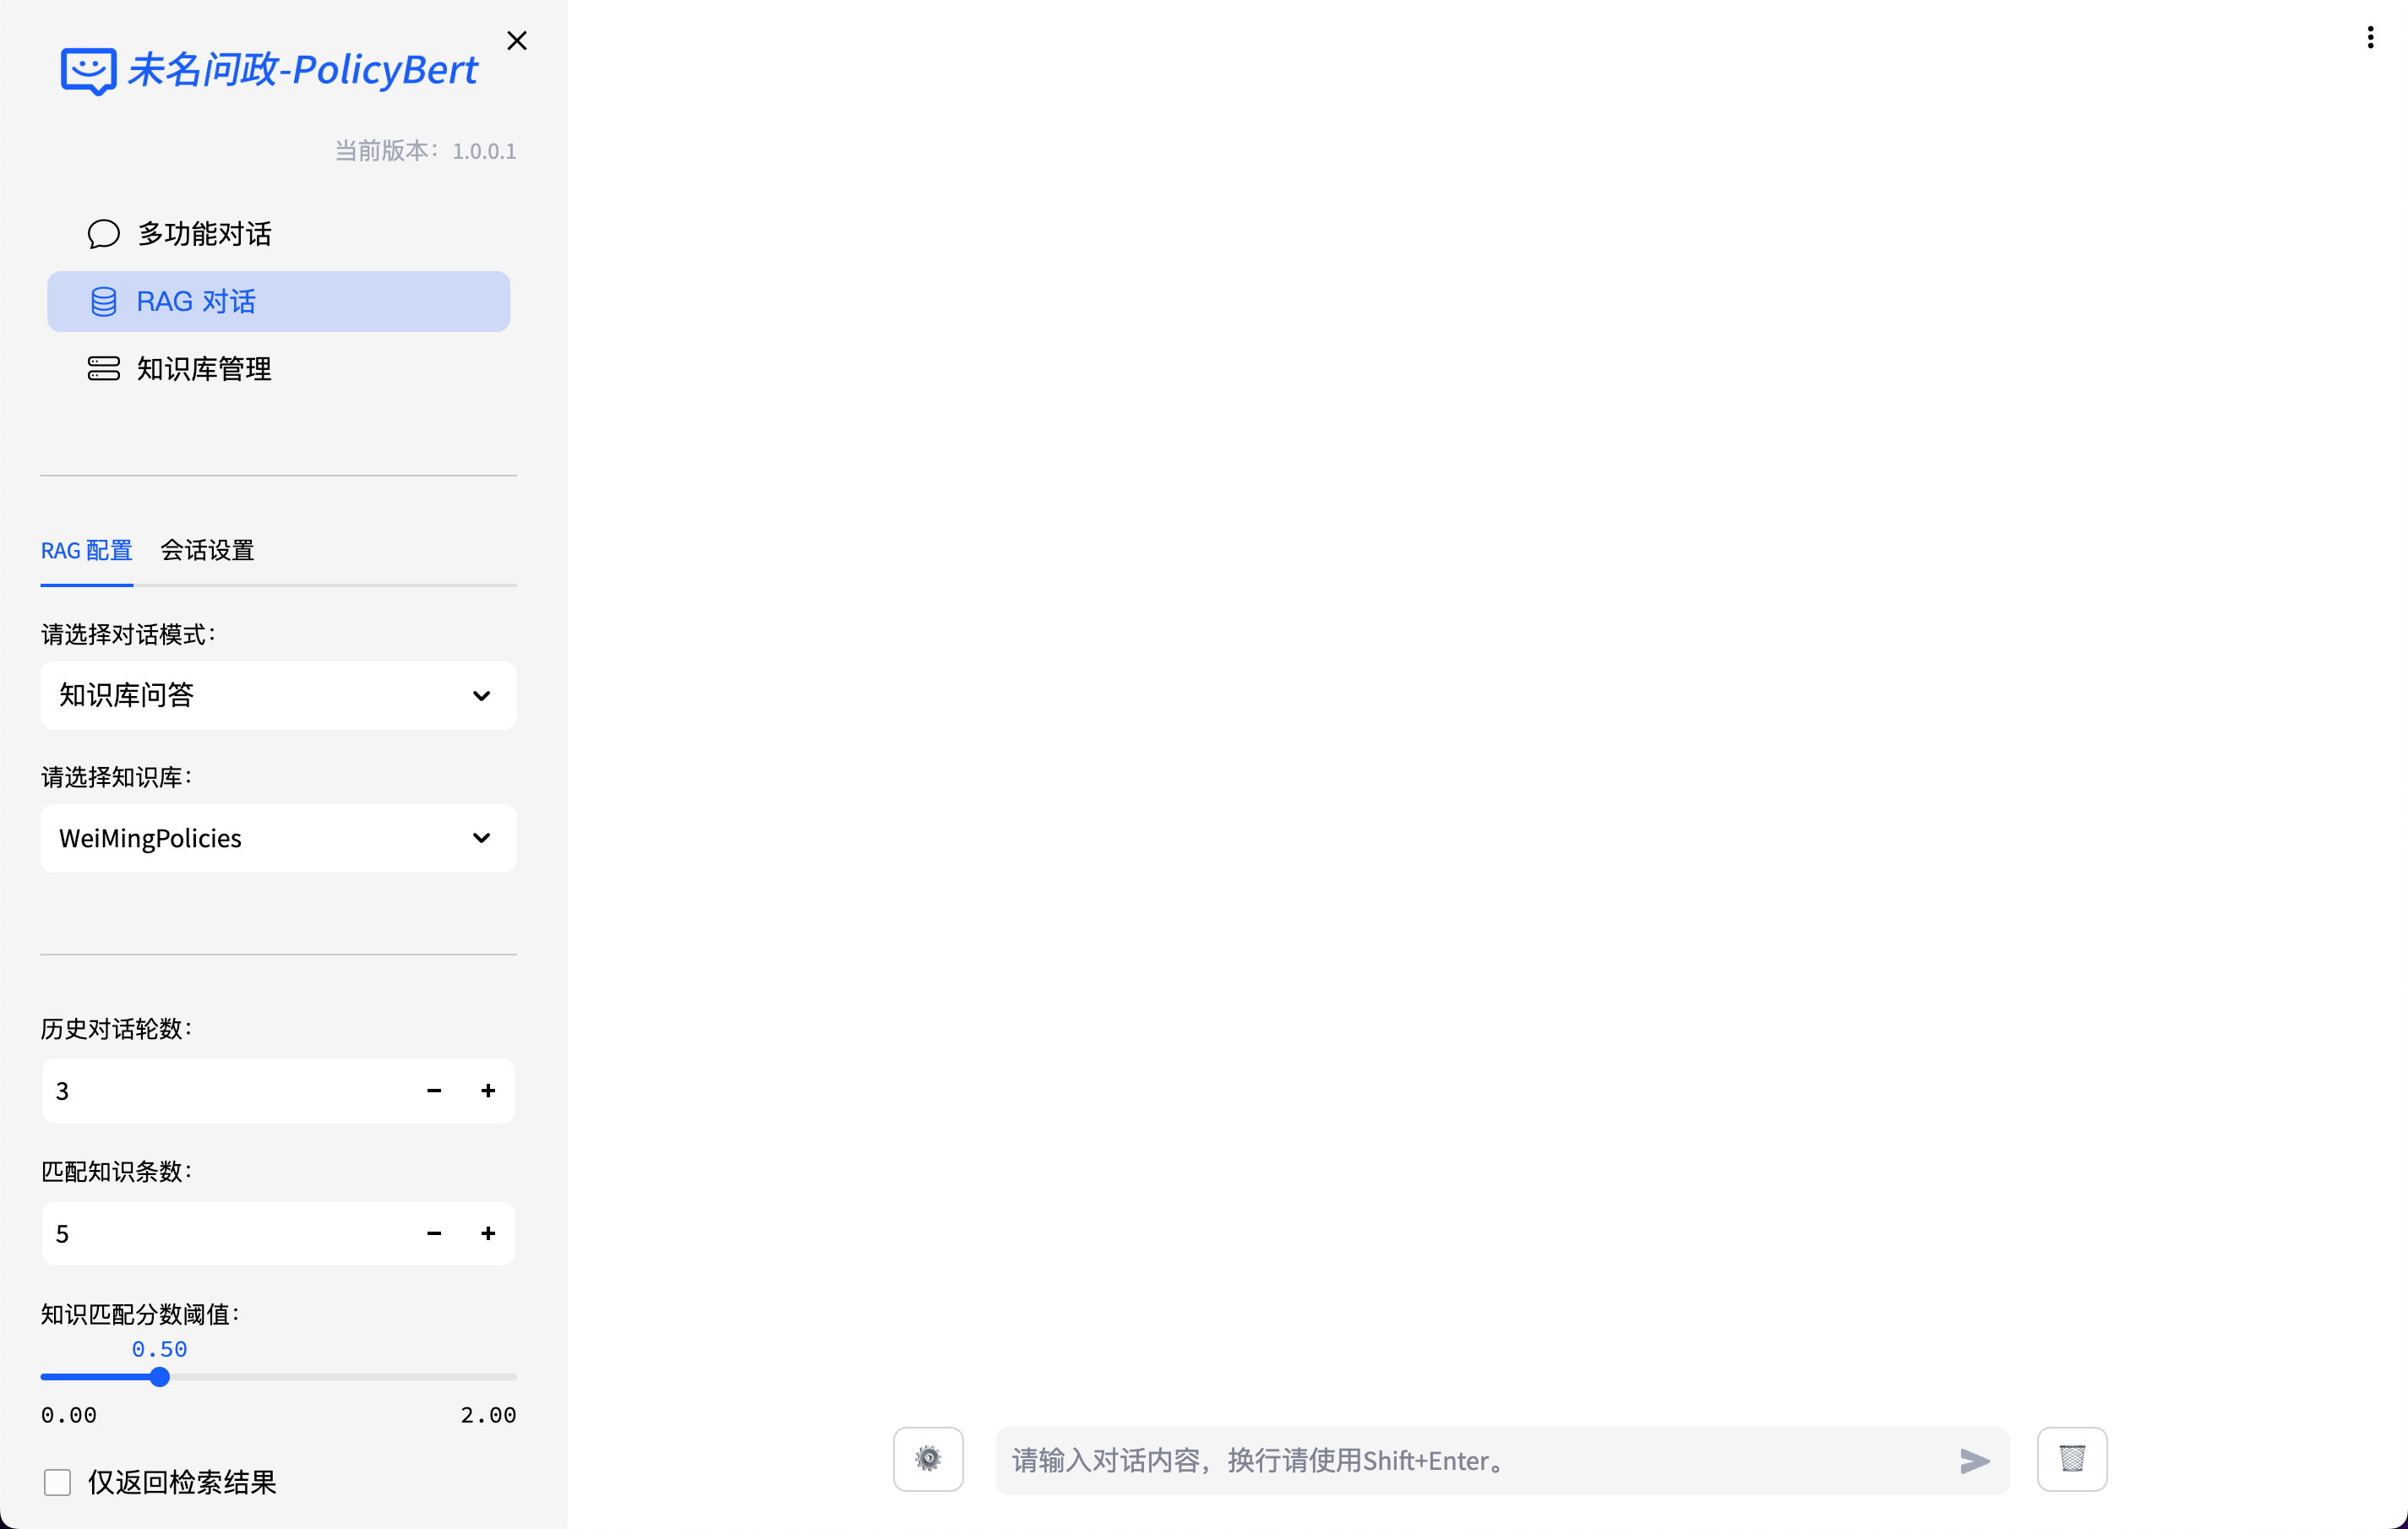
\includegraphics[width=0.8\textwidth]{./images/home_page.png}
    \caption{未名问政 RAG 系统首页界面。界面左侧为参数配置区域,支持设置对话模式、知识库来源、历史轮数、匹配条数及知识匹配分数阈值,右侧为对话窗口区域,用于显示模型响应结果。该系统通过图形化界面提供了灵活高效的RAG任务配置方式。}
    \label{fig:home_page}
\end{figure}

如图\ref{fig:system_running},未名问政RAG在“RAG 对话”模式下提供了图形化的参数配置与实时问答界面。右侧展示了用户提问(如“什么是数据基础制度体系?”)、知识库匹配结果(下拉列表形式展现检索到的原文段落)及模型最终生成的回答。该对话结果展现了未名问政RAG系统在政策文本问答任务中的优异表现。系统准确理解了用户提出的“什么是数据基础制度体系?”这一问题,并结合知识库中的相关内容,生成了逻辑清晰、内容详实的回答。回答不仅涵盖了数据基础制度体系的定义,还详细阐述了其包含的四个方面的制度内容,条理分明,层次清晰,充分体现了系统在检索增强生成(RAG)任务中的强大能力。此外,回答语言流畅自然,专业性强,能够很好地满足用户对政策解读的需求,展现了系统在政务智能问答场景中的实际应用价值。

\begin{figure}[H]
    \centering
    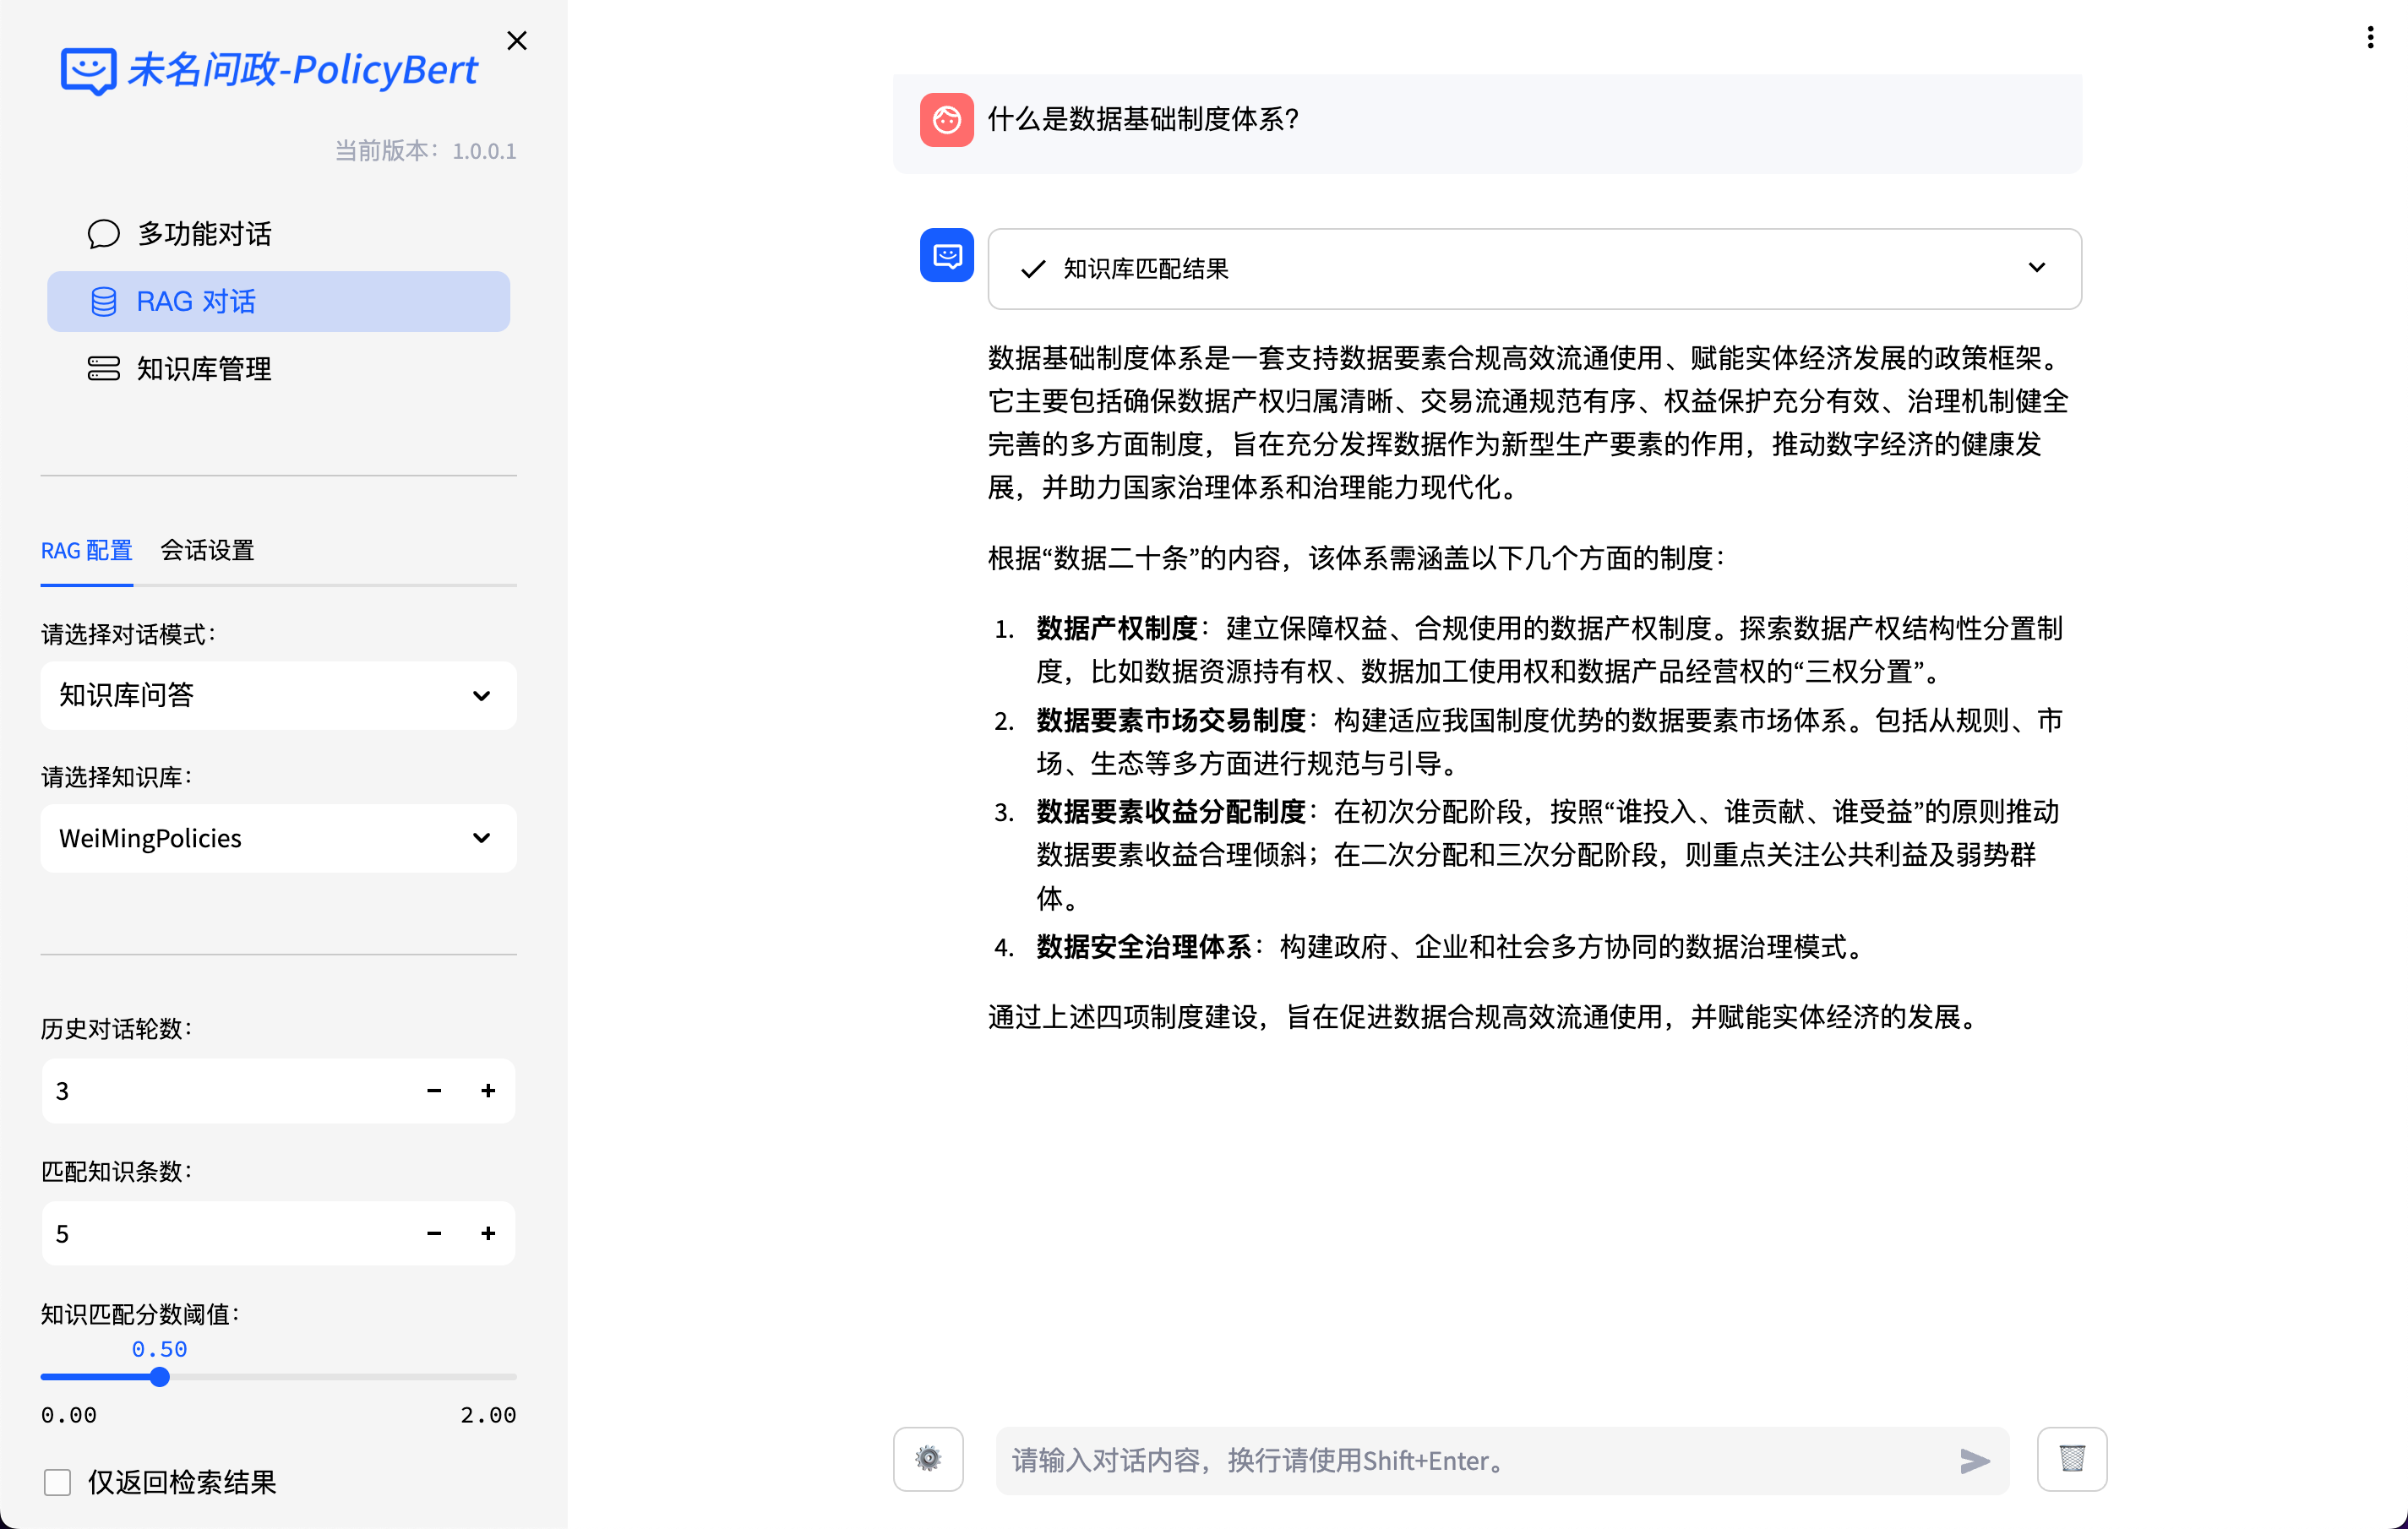
\includegraphics[width=0.8\textwidth]{./images/system_running.png}
    \caption{未名问政 RAG 系统对话界面。左侧为参数配置区域,右侧为对话窗口区域。用户可在输入框中输入问题,系统将根据设置的参数进行检索与生成。}
    \label{fig:system_running}
\end{figure}

在图\ref{fig:system_retrieve_only}中的对话中,用户启用了“仅返回检索结果”功能,系统准确地从知识库中检索出了与用户问题“什么是数据基础制度体系?”高度相关的政策文本片段。检索结果内容详实,涵盖了数据基础制度体系的核心定义及其在政策框架中的重要作用,并引用了权威来源,确保了信息的可靠性和专业性。从结果来看,该功能能够有效地将用户问题与知识库中的相关内容进行精准匹配,避免了生成式回答可能带来的信息偏差或冗余问题,特别适用于需要直接引用政策原文或获取权威信息的场景。这种检索增强的方式不仅提升了系统的实用性和可信度,也为用户提供了更高效的政策信息获取途径。

\begin{figure}[H]
    \centering
    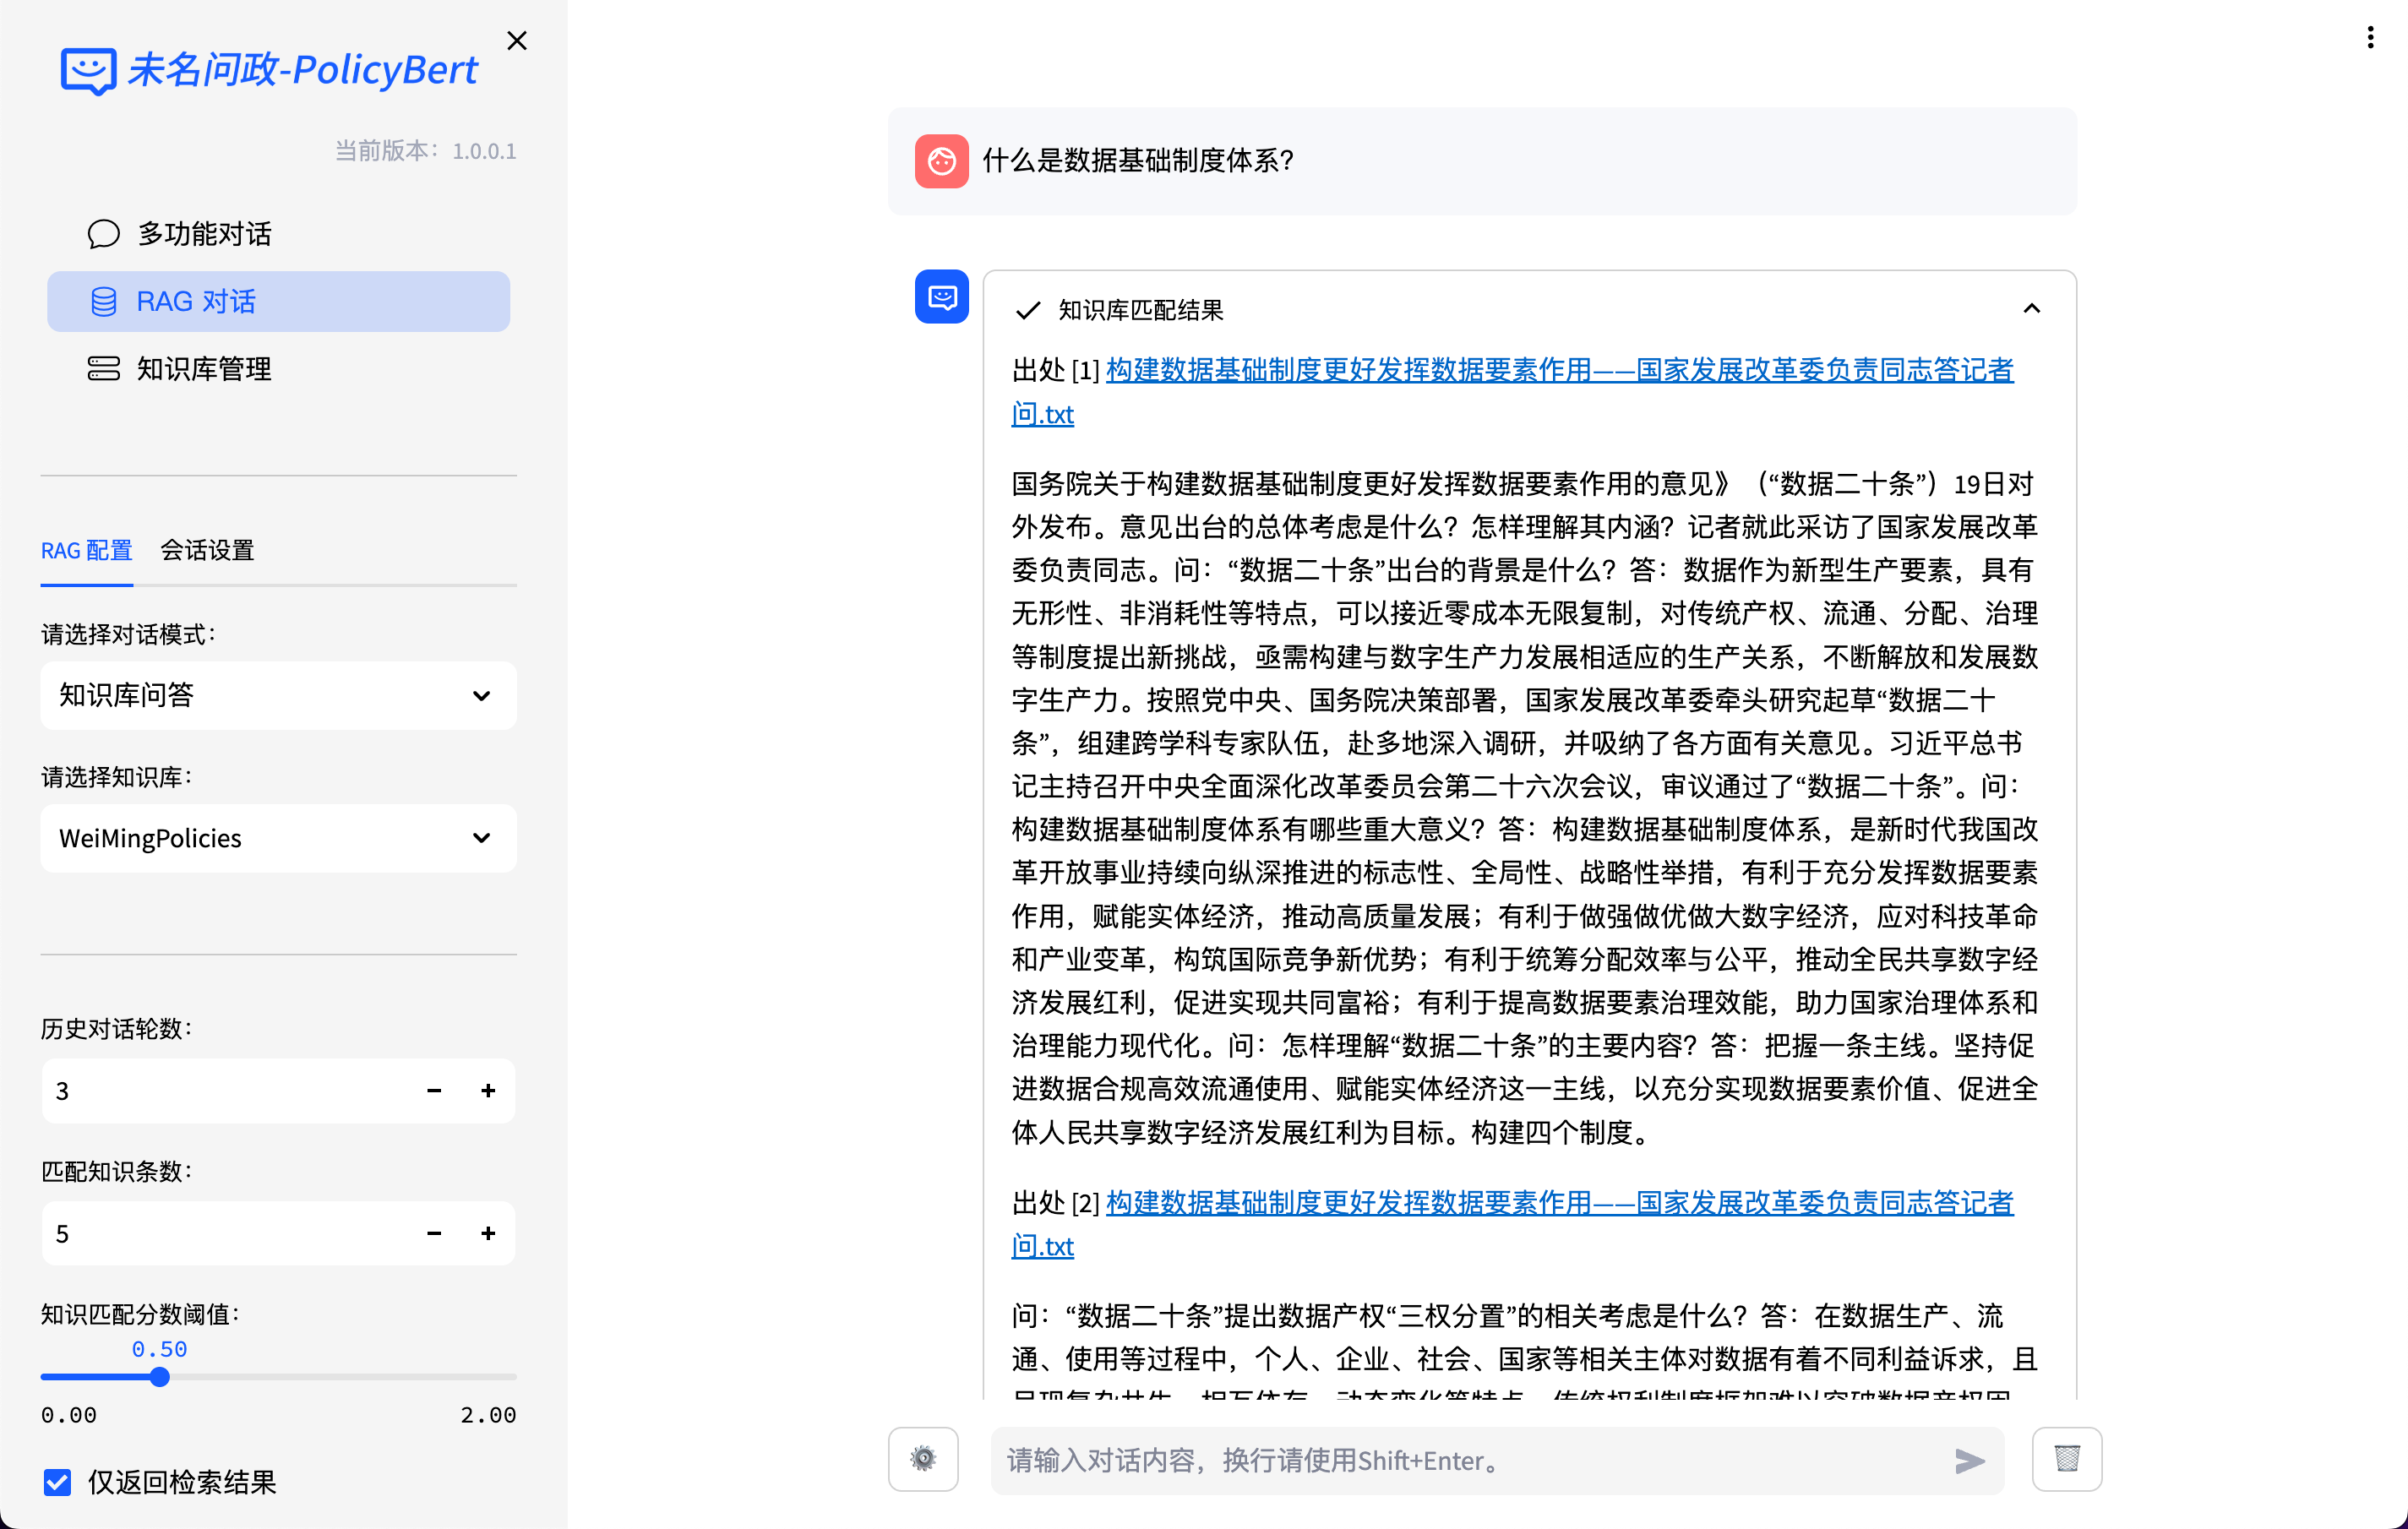
\includegraphics[width=0.8\textwidth]{./images/system_retrieve_only.png}
    \caption{未名问政 RAG 系统检索结果界面。用户使用“仅返回检索结果”功能,系统准确地从知识库中检索出了与用户问题“什么是数据基础制度体系?”高度相关的政策文本片段。}
    \label{fig:system_retrieve_only}
\end{figure}

\subsubsection{知识库管理}
如图\ref{fig:kb_manage_1}和\ref{fig:kb_manage_2}所示,未名问政RAG系统的知识库管理模块允许用户对知识库进行增删改查操作。用户可以通过“上传知识文件”功能,将新的政策文本片段添加至知识库中,以便后续检索与生成使用。同时,系统支持对已有知识进行编辑和删除操作,确保知识库内容的及时更新与维护。此外,用户还可以通过“查看知识”功能,快速浏览当前知识库中的所有条目,方便进行信息检索与管理。该模块的设计旨在提升系统的灵活性与可扩展性,使其能够适应不断变化的政策环境与用户需求。

\begin{figure}[H]
    \centering
    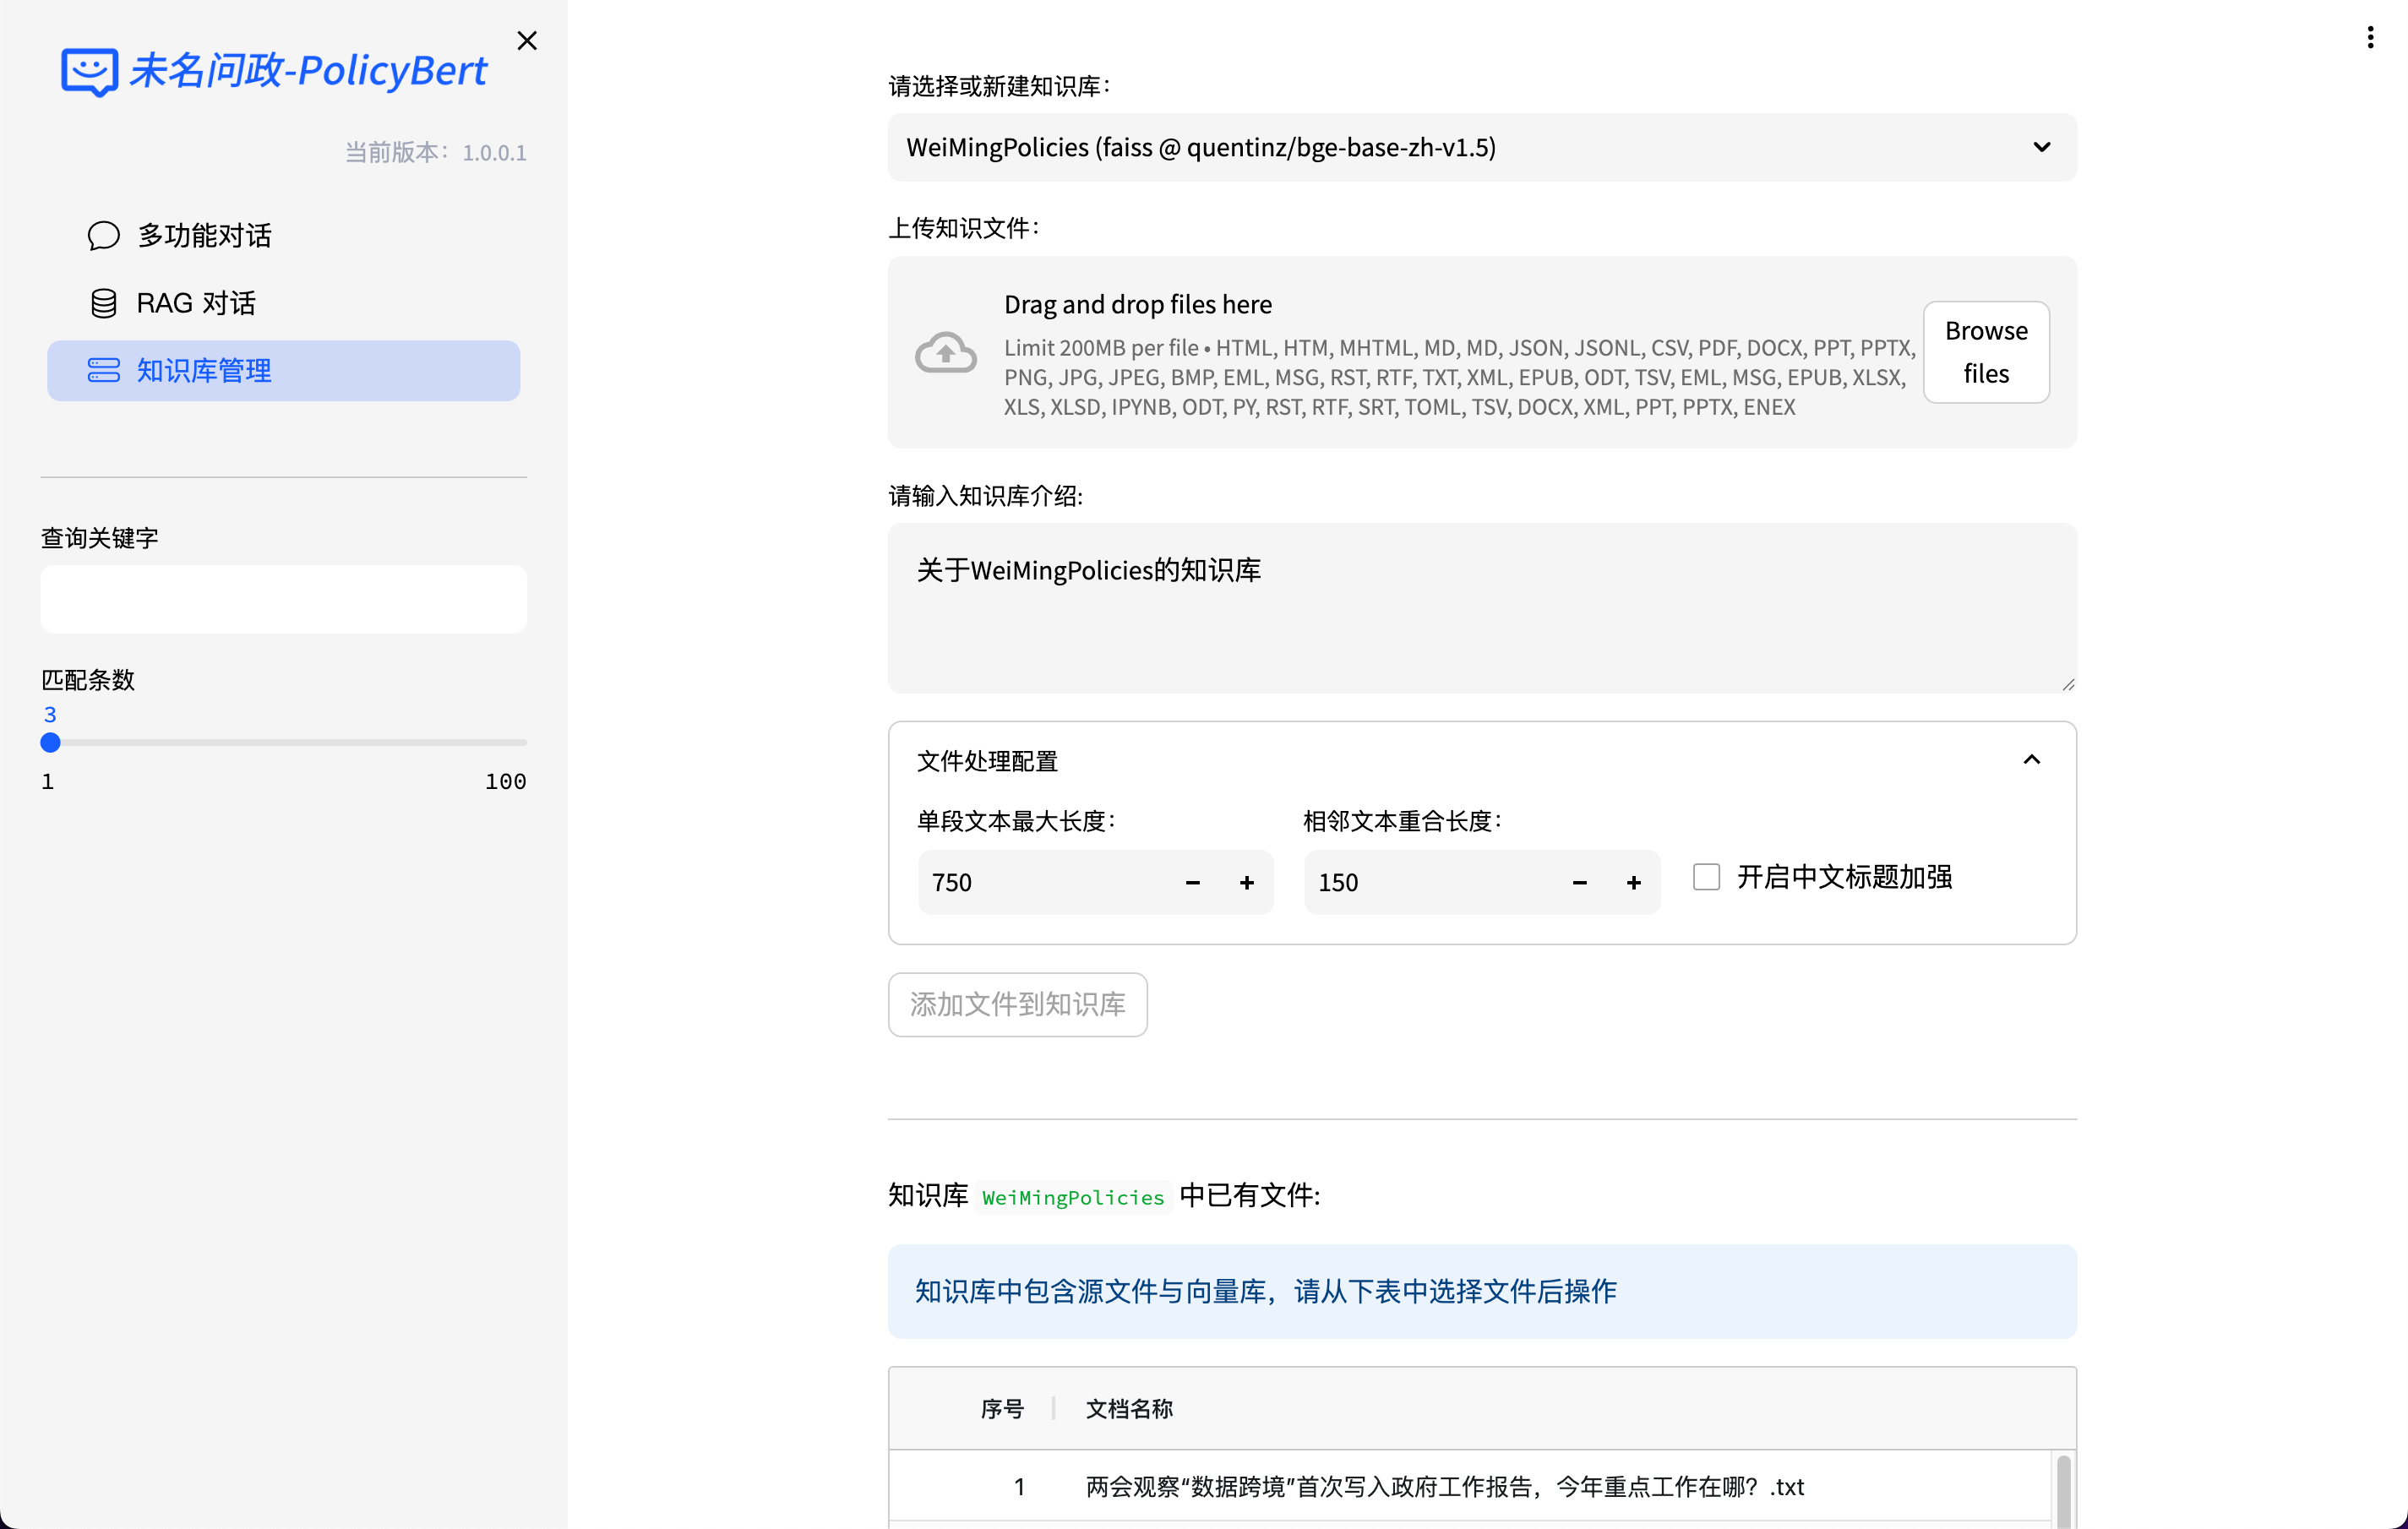
\includegraphics[width=0.8\textwidth]{./images/kb_manage_1.png}
    \caption{未名问政 RAG 系统知识库管理界面。用户可以通过“上传知识文件”功能,将新的政策文本片段添加至知识库中,以便后续检索与生成使用。}
    \label{fig:kb_manage_1}
\end{figure}

\begin{figure}[H]
    \centering
    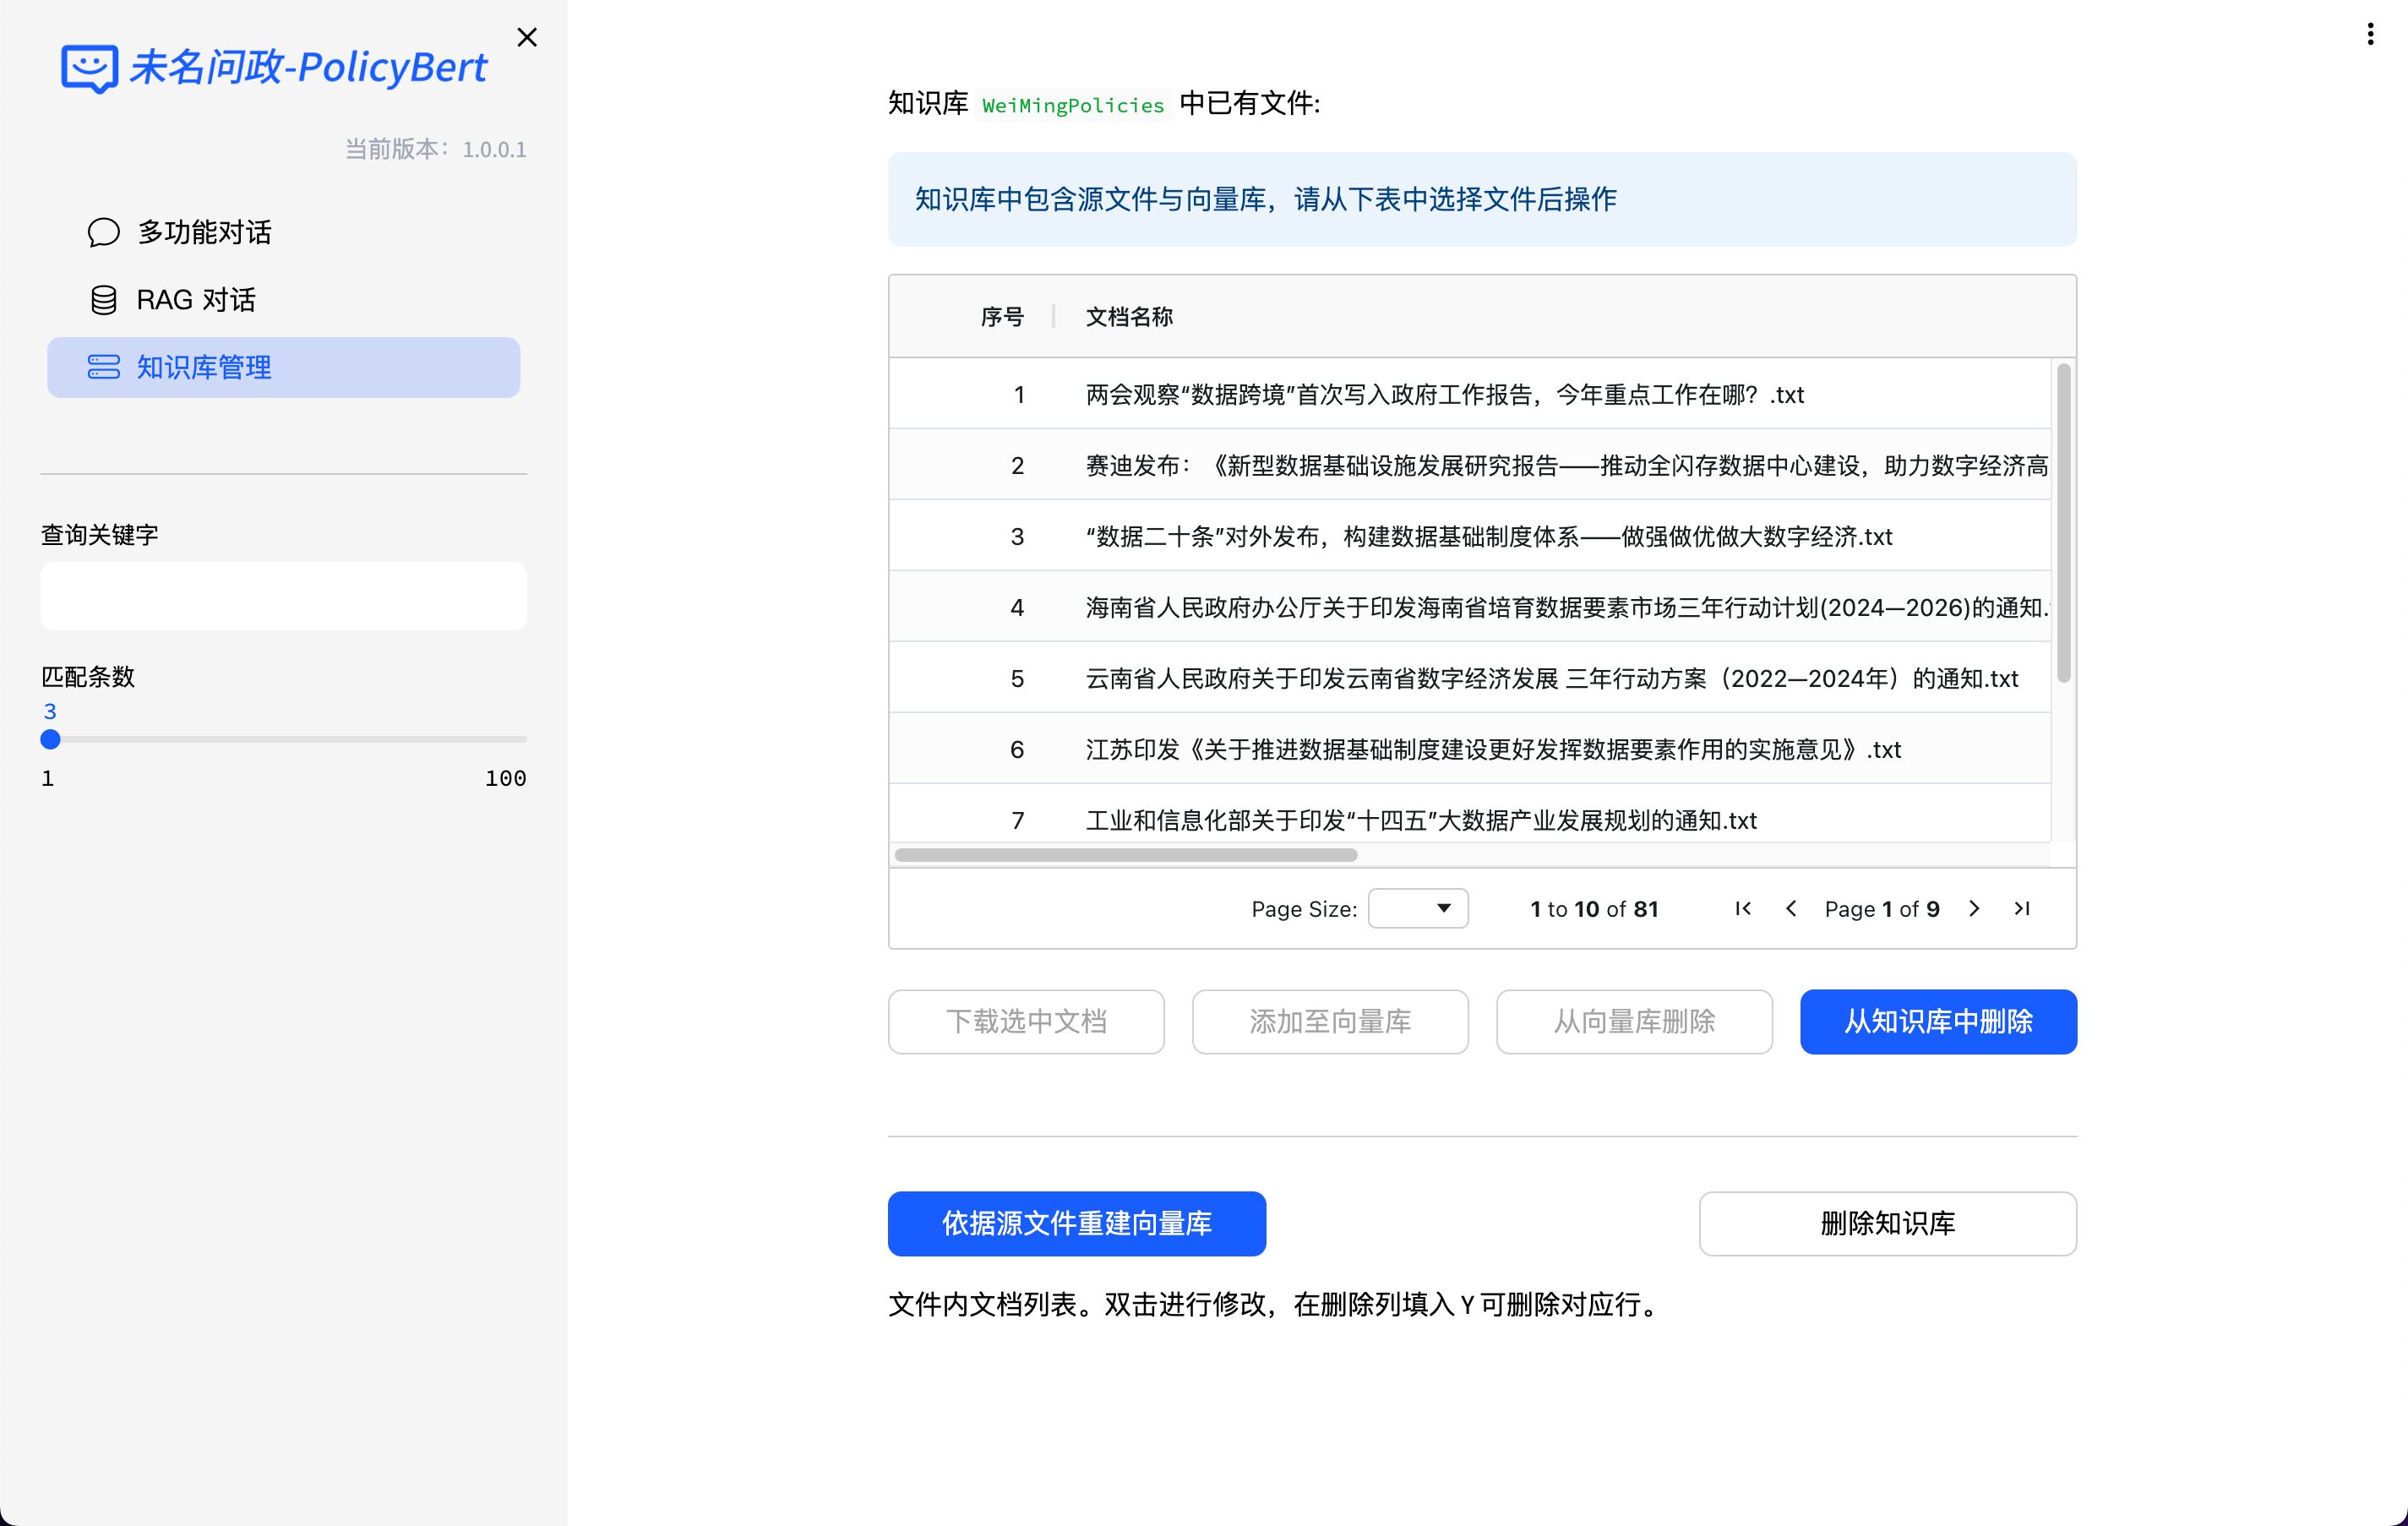
\includegraphics[width=0.8\textwidth]{./images/kb_manage_2.png}
    \caption{未名问政 RAG 系统知识库管理界面。用户可以通过“查看知识”功能,快速浏览当前知识库中的所有条目,方便进行信息检索与管理。}
    \label{fig:kb_manage_2}
\end{figure}

\section{总结与展望}
\subsection{结论与总结}
本文提出了一种基于融合式中文编码模型的文本编码器,旨在提升中文政策文本的语义理解与生成能力。通过对比不同的融合方法(门控机制、多头注意力机制)与分词策略(n-gram、Hanlp),我们验证了融合式模型在中文政策文本处理中的有效性。实验结果表明,使用Hanlp分词的模型在所有融合方法中表现最好,达到了0.9132的准确率。
此外,我们还构建了两个适用于中文政策文本的NSP任务数据集(PolicySM-1和PolicySM-2),并在这两个数据集上进行了模型微调。实验结果显示,使用多头注意力机制的模型在NSP任务中表现最佳,达到了0.9325的准确率。
最后,基于微调后的模型,我们构建了一个基于检索增强生成(RAG)机制的智能问答系统“未名问政”,实现了从文本检索到问答生成的全流程部署。该系统具备部署灵活、响应快速、扩展便捷等特点,适用于政务智能问答、政策知识库构建与自动解读等场景。

\subsection{不足与展望}
尽管本文提出的PolicyBERT模型在中文政策文本的语义理解与生成任务中取得了显著的性能提升,但仍存在一些不足之处需要进一步改进。首先,模型的训练和评估主要基于特定领域的政策文本数据集,虽然在该领域表现优异,但其在其他领域的泛化能力尚未得到充分验证。未来可以尝试扩展数据集的覆盖范围,探索模型在多领域文本处理中的适用性。

本文采用了HanLP分词工具和基于门控机制与多头注意力机制的融合方法,尽管在实验中表现出色,但分词错误和词表构建的局限性可能对模型性能产生一定影响。未来可以尝试引入更先进的分词技术或预训练方法,以进一步提升模型对中文语言特性的适应能力。

此外,模型的训练和评估主要集中在NSP任务上,虽然在该任务上取得了良好的效果,但在其他下游任务(如文本分类、情感分析等)上的表现尚未得到充分验证。未来可以尝试构建更多的下游任务数据集,并对模型进行多任务学习,以提升其在不同任务上的泛化能力。

由于缺少大规模预训练语料,模型无法进行在大规模语料上从零开始的预训练,导致模型在一些复杂的语义理解任务上仍然存在一定的局限性。未来可以尝试引入更多的预训练数据,或结合其他预训练模型进行迁移学习,以提升模型的性能。

最后,模型的计算复杂度较高,尤其是在多头注意力机制的融合过程中,对硬件资源的需求较大。这在一定程度上限制了模型在资源受限环境中的应用。未来可以尝试优化模型结构或引入轻量化技术,如知识蒸馏或模型剪枝,以降低计算成本并提升部署效率。


% \newpage
\bibliographystyle{unsrt}
\bibliography{references}

% \section{附录}

\newpage
\section{致谢}

感谢导师的悉心指导和支持,感谢同学们的帮助与鼓励,感谢家人对我的理解与支持。

\newpage
\section{北京大学学位论文原创性声明和使用授权说明}

\vspace{1em} % 添加空行

\begin{center}
    \textbf{原创性声明}
\end{center}

\vspace{1em} % 添加空行

本人郑重声明:所呈交的学位论文,是本人在导师的指导下,独立进行研究工作所取得的成果。除文中已经注明引用的内容外,本论文不含任何其他个人或集体已经发表或撰写过的作品或成果。对本文的研究做出重要贡献的个人和集体,均已在文中以明确方式标明。本声明的法律结果由本人承担。

\vspace{4em} % 添加空行

\hfill 论文作者签名:\underline{\hspace{3cm}} 

\vspace{2em} % 添加空行

\hfill 日期:\underline{\hspace{2cm}} 年 \underline{\hspace{1cm}} 月 \underline{\hspace{1cm}} 日

\vspace{2em} % 添加空行

\begin{center}
    \textbf{学位论文使用授权说明}
\end{center}

\vspace{1em} % 添加空行

本人完全了解北京大学关于收集、保存、使用学位论文的规定,即:
\begin{itemize}
    \item 按照学校要求提交学位论文的印刷本和电子版本;
    \item 学校有权保存学位论文的印刷本和电子版,并提供目录检索与阅览服务,在校园网上提供服务;
    \item 学校可以采用影印、缩印、数字化或其它复制手段保存论文。
\end{itemize}

\vspace{2em} % 添加空行

\hfill 论文作者签名:\underline{\hspace{3cm}} \hspace{2em} 导师签名:\underline{\hspace{3cm}}

\vspace{1em} % 添加空行

\hfill 日期:\underline{\hspace{2cm}} 年 \underline{\hspace{1cm}} 月 \underline{\hspace{1cm}} 日      


\end{document}